% vim:tw=120:sw=2:enc=utf-8
\documentclass[a4paper,12pt,titlepage]{book}
% vim:tw=120:sw=2:enc=utf-8

% csomag opciók
\def\magyarOptions{frenchspacing=yes,activeprefix=grave}

% csomagok
\usepackage[utf8]{inputenc}
\usepackage{t1enc}
\usepackage[english,magyar]{babel}
\usepackage[dvips]{graphicx}
\usepackage{graphics}
\usepackage{graphicx}
\usepackage{fancyvrb}
%\usepackage{amsrefs}
\usepackage{amsmath}
\usepackage{alltt}
\usepackage{verbatim}
\usepackage{booktabs}
\usepackage{paralist}
\usepackage{fancyhdr}
\usepackage{xspace}
\usepackage{listings}
\usepackage{amsmath}
\usepackage{amssymb}

% makrók
\makeatletter
\def\Ifnopdflatex{\csname @ifundefined\endcsname{pdfcompresslevel}}
\makeatother

% méretek
%\addtolength{\voffset}{-1cm}
\addtolength{\textheight}{2cm}
\addtolength{\hoffset}{-1.2cm}
\addtolength{\textwidth}{2.4cm}
\setlength{\headheight}{16pt}

\renewcommand{\headrulewidth}{0.5pt}
\renewcommand{\footrulewidth}{0pt}

\addtolength{\oddsidemargin}{9mm}
\addtolength{\evensidemargin}{-7mm}

\pagestyle{fancy}
\fancyhf{}
\fancyhead[LE,RO]{\sffamily\thepage}%
\fancyhead[LO]{\sffamily\sc\nouppercase{\rightmark}}%
\fancyhead[RE]{\sffamily\sc\nouppercase{\leftmark}}%


\fancypagestyle{plain}{\fancyhf{}\renewcommand{\headrulewidth}{0pt}}

\newcounter{fejezet}
\makeatletter
\renewcommand{\chaptermark}[1]{\markboth{\ifnum \thechapter > 0
   \ifnum \c@fejezet = 1
          \thechapter.\ \chaptername.\ %
	     \fi
 \fi#1}{}
}

\renewcommand{\sectionmark}[1]{\markright{\thesection.\ #1}}
\makeatother


\newcommand{\chaptern}[1]{
\setcounter{fejezet}{0}%
\chapter*{#1}%
\addcontentsline{toc}{chapter}{#1}%
\chaptermark{#1}%
}

\newcommand{\chaptery}[1]{
\setcounter{fejezet}{1}%
\chapter{#1}%
}


\makeatletter
\def\cleardoublepage{\clearpage\if@twoside \ifodd\c@page\else
\hbox{}
\thispagestyle{empty}
\newpage
\if@twocolumn\hbox{}\nepage\fi\fi\fi}
\makeatother

\clearpage{\thispagestyle{empty}\cleardoublepage}
\makeatletter
\newcommand{\elv}{\leavevmode\nobreak-\hskip\z@skip}
\makeatother

%%%
% Magyar tipográfiai előírások
%%%

\baselineskip=0pt
\parskip=0pt


%%%%%%

\newcommand{\xml}{\textsc{xml}\xspace}

\newcommand*{\utbeh}{\hspace*{3mm}}

\newcommand{\ut}[1]{\hspace*{3mm}\mbox{\vspace{2mm}\texttt{#1}\vspace{2mm}}}

\DefineVerbatimEnvironment%
{VerbExampleNum}{Verbatim}
{numbers=left,xleftmargin=8mm,xrightmargin=8mm}

\DefineVerbatimEnvironment%
{VerbExample}{Verbatim}
{xleftmargin=5mm,xrightmargin=5mm}


%% \title{Programozási környezet jegyzet}
%% \author{Tóth László Attila}
%% \date{2007. június 1.}

%% \addtolength{\oddsidemargin}{9mm}
%% \addtolength{\evensidemargin}{-7mm}

%% \hyphenation{a-mely-re}

\begin{document}

  %% \documentclass[a4paper,final,12pt]{book}

%% % vim:tw=120:sw=2:enc=utf-8

% csomag opciók
\def\magyarOptions{frenchspacing=yes,activeprefix=grave}

% csomagok
\usepackage[utf8]{inputenc}
\usepackage{t1enc}
\usepackage[english,magyar]{babel}
\usepackage[dvips]{graphicx}
\usepackage{graphics}
\usepackage{graphicx}
\usepackage{fancyvrb}
%\usepackage{amsrefs}
\usepackage{amsmath}
\usepackage{alltt}
\usepackage{verbatim}
\usepackage{booktabs}
\usepackage{paralist}
\usepackage{fancyhdr}
\usepackage{xspace}
\usepackage{listings}
\usepackage{amsmath}
\usepackage{amssymb}

% makrók
\makeatletter
\def\Ifnopdflatex{\csname @ifundefined\endcsname{pdfcompresslevel}}
\makeatother

% méretek
%\addtolength{\voffset}{-1cm}
\addtolength{\textheight}{2cm}
\addtolength{\hoffset}{-1.2cm}
\addtolength{\textwidth}{2.4cm}
\setlength{\headheight}{16pt}

\renewcommand{\headrulewidth}{0.5pt}
\renewcommand{\footrulewidth}{0pt}

\addtolength{\oddsidemargin}{9mm}
\addtolength{\evensidemargin}{-7mm}

\pagestyle{fancy}
\fancyhf{}
\fancyhead[LE,RO]{\sffamily\thepage}%
\fancyhead[LO]{\sffamily\sc\nouppercase{\rightmark}}%
\fancyhead[RE]{\sffamily\sc\nouppercase{\leftmark}}%


\fancypagestyle{plain}{\fancyhf{}\renewcommand{\headrulewidth}{0pt}}

\newcounter{fejezet}
\makeatletter
\renewcommand{\chaptermark}[1]{\markboth{\ifnum \thechapter > 0
   \ifnum \c@fejezet = 1
          \thechapter.\ \chaptername.\ %
	     \fi
 \fi#1}{}
}

\renewcommand{\sectionmark}[1]{\markright{\thesection.\ #1}}
\makeatother


\newcommand{\chaptern}[1]{
\setcounter{fejezet}{0}%
\chapter*{#1}%
\addcontentsline{toc}{chapter}{#1}%
\chaptermark{#1}%
}

\newcommand{\chaptery}[1]{
\setcounter{fejezet}{1}%
\chapter{#1}%
}


\makeatletter
\def\cleardoublepage{\clearpage\if@twoside \ifodd\c@page\else
\hbox{}
\thispagestyle{empty}
\newpage
\if@twocolumn\hbox{}\nepage\fi\fi\fi}
\makeatother

\clearpage{\thispagestyle{empty}\cleardoublepage}
\makeatletter
\newcommand{\elv}{\leavevmode\nobreak-\hskip\z@skip}
\makeatother

%%%
% Magyar tipográfiai előírások
%%%

\baselineskip=0pt
\parskip=0pt


%%%%%%

\newcommand{\xml}{\textsc{xml}\xspace}

\newcommand*{\utbeh}{\hspace*{3mm}}

\newcommand{\ut}[1]{\hspace*{3mm}\mbox{\vspace{2mm}\texttt{#1}\vspace{2mm}}}

\DefineVerbatimEnvironment%
{VerbExampleNum}{Verbatim}
{numbers=left,xleftmargin=8mm,xrightmargin=8mm}

\DefineVerbatimEnvironment%
{VerbExample}{Verbatim}
{xleftmargin=5mm,xrightmargin=5mm}



\author{Tóth László Attila}
\title{Programozási Környezet jegyzet}
% TODO: aktualis datum helyett mas. Utolso modositas ideje?
%\date{2007. szeptember 10.}
%%\begin{document}
\makeatletter
\begin{titlepage}%
  \let\footnotesize\small
  \let\footnoterule\relax
  \begin{center}%
    
\includegraphics[width=0.2\textwidth]{elte.eps}\hskip 3em%
    \parbox[b][3cm][c]{10cm}{%
      \begin{center}%
	Eötvös Loránd Tudományegyetem\\
	Informatikai Kar\\
	Programozáselmélet és Szoftvertechnológia Tanszék\end{center}}  
    \vskip 1em%
    \hrule 
    \vspace{70mm}%
	  {\LARGE \bf \@title \par}%
	   \vskip 2em%
		  {\large
		    \lineskip .75em%
		     \begin{tabular}[t]{ll}%
		       Készítette: & \@author
			\end{tabular}\par}%
  \end{center}%\\partial   
  \vskip 12em
  \vspace{20mm}
  \hskip 2em Budapest, \@date
  %\vskip 8em
  \vfill\null
\end{titlepage}%  
\makeatother
%%\end{document}

% Local Variables:
% fill-column: 120
% mode: latex
% End:

  \pagestyle{fancy}

  \frontmatter
  \tableofcontents
  
  \mainmatter
  \newpage
  \chaptern{Bevezetés}
\label{cha:bevezetes}

A \emph{Programozási környezet} tárgy keretein belül a \textsc{html} alapjait,
\textsc{unix} shell szkripteket (konkrétan Linuxokon Bash-t) valamint
\textsc{vms}-t oktatunk. E jegyzet az előbbi kettőről szól, a \textsc{html}
alapjairól és minimális \textsc{css}-ről, valamint részletesen a Bash szkriptek
készítéséről.

A jegyzet felépítése a következő: a \textsc{html}-ről, annak is az
\textsc{xhtml} változatáról egyetlen fejezetben a -- \aref{cha:html}.\
fejezetben --, a Linuxról és a parancssorról pedig a többi fejezetben. A Linux
és a Bash alapjairól szól \aref{cha:linux}.\ és \aref{cha:shell}.,
 a szövegfeldogolzásban
használható programokról, a szűrőkről \aref{cha:szűrők}., a
környezeti változókról -- használatukról és a lényegesebb előre definiáltak
jelentéséről \aref{cha:env-vars}., a vezérlési szerkezetekről -- elágazás,
szekvencia és ciklus -- \aref{cha:vez-szerk}., a reguláris kifejezésekről
\aref{cha:regex}., végezetül az awk-ról, és egyéb, az előző fejezetekben el nem
hangzott lehetőségekről \aref{cha:others}.\ fejezetben.

Néhány fejezet elején szerepel történeti áttekintés, amely csupán tájékoztató
jellegű és nem mindig pontos.


% Local Variables:
% fill-column: 80
% mode: latex
% End:

  

\chaptery{A \textsc{html}, \textsc{xhtml} és a \textsc{css}}%
\label{cha:html}

A hálózat elterjedésével lehetővé vált az információk különböző oldalakon
történő tárolása, amelyhez idővel szükségessé vált egy ezt segítő
jelölésrendszer kialakítása. Ezáltal már nem pusztán szöveges információt
lehetett átadni, hanem azt is, hogy ezen szöveg melyik része milyen szerepet
tölt be, ráadásul nagyon könnyen lehetett szerkeszteni az ilyen oldalakat. Ezt
teszi lehetővé a \textsc{html} \cite{html}, amely a 90-es években jelent meg és
terjedt el. A \textsc{html} egy betűszó, a \emph{Hypertext Markup Language}
rövidítése, vagyis egy olyan jelölő nyelv, amely segítségével az oldalak között
lehet lépegetni.

Ma is \textsc{html}-ben készül a legtöbb (web)oldal, azonban már nem statikusak,
valamilyen program készíti el akkor, amikor a felhasználó a böngészője
segítségével lekérdezi. Sőt, a letöltött oldal is dinamikus, hiszen JavaScript
segítségével megváltoztatható az oldal kinézete, vagy éppen az űrlapok mezőit
már a böngészőben le lehet ellenőrizni, hogy a felhasználó tudja, melyiket kell
még javítania. Ma már egyre jobban terjed az a megoldás is, amit szintén
JavaScript-tel oldanak meg, hogy a letöltött oldal egyes részei úgy frissülnek,
hogy egy JavaScript program kérdezi le az adatokat, a felhasználónak nem kell az
oldalt frissítenie, vagy másik oldalra lépnie (\textsc{ajax} \cite{ajax}).

Mára nagyon sok hibás weboldal készült, ahol a szerkezetet jelző címkék
sorrendje helytelen, vagy egyszerűen nincs is. Részben ezt hivatott kiküszöbölni
a \textsc{html} egyik változata, az \textsc{xhtml} \cite{xhtml1,xhtml11}, amely
szigorúan veszi a jelöléseket, ezáltal egy program is könnyebben feldolgozhatja,
és átláthatóbb is.

Az eredeti változatot (\textsc{html 4}) ma is fejlesztik, a következő változatra
elkészült egy javaslat, amely sajnos figyelmen kívül hagyja az \texttt{xhtml}
nyújtotta előnyeket.


\section{A(z \textsc{x})\textsc{html}}

Minden szónál többet ér egy példa, így álljon itt egy példa minimális
\textsc{xhtml} 1.1-es oldalra - amely megfelel a legújabb \textsc{w3c}
ajánlásnak \cite{html}, és \aref{fig:xhtml-minimal}.\ ábrán látható.

\begin{figure}[tbh]\center
\begin{VerbExampleNum}
<?xml version="1.0" encoding="ISO-8859-2"?>
<!DOCTYPE html PUBLIC "-//W3C//DTD XHTML 1.1//EN"
"http://www.w3.org/TR/xhtml11/DTD/xhtml11.dtd">
<html xmlns="http://www.w3.org/1999/xhtml" xml:lang="hu">
<head><title>Ez a cím</title></head>
<body>
Itt van valamilyen szöveg
</body>
</html>
\end{VerbExampleNum}
   \caption{Egy minimális \textsc{xhtml} oldal}
  \label{fig:xhtml-minimal}
\end{figure}


Az első sor jelzi, hogy ez nem csupán egy \textsc{html} oldal, hanem egy olyan
dokumentum,
amely megfelel az XML szabványnak \cite{xml} is. A második és harmadik sor még
mindig nem része magának a \textsc{html} oldalnak, hanem annak szerkezetét
definiálja: azt, hogy hol van a dokumentumtípust leíró definíció, és számos
kapcsolódó információt.

Látható, hogy különböző jelentésű szavak szerepelnek kacsacsőrök
között. Mindegyik ilyen szó egy-egy címke (angolul: tag), amely a dokumentum
szerkezetét határozza meg. Szerepelnek nevek (pl.\ \texttt{html}, \texttt{head},
\texttt{title}), és
a névhez tartozó tulajdonságok is, ilyen például az \texttt{xml:lang}, mely a
dokumentum nyelvét határozza meg. A tulajdonságok vagy attribútumok mindegyike
egy névből, és egy attól egyenlőségjellel elválasztott értékből áll. Az
értékeket idézőjelek közé kell tenni, ugyanis szerepelhet bennük szóköz, és
ezáltal egyértelmű, hogy mettől meddig tartanak.


\section{A \textsc{html} elemek}
Az előzőek figyelembe vételével már könnyen definiálhatóak a \textsc{html} és
\textsc{xhtml} dokumentumok építőkövei, a \textsc{html} elemek (element). Ezek
mindegyike egy névből áll, valamint tulajdonságokból (attributes). A nevet
szokták címkének (tag) hívni. Mindegyiket le kell zárni, vagyis például a
\texttt{html} elemnek van egy nyitó és egy lezáró fele is: \verb|<html>| és
\verb|</html>|; a lezáró rész a nyitóval azonos, azonban csak a nevet
tartalmazza, amelyet egy perjel előz meg.

Az elemek egymásba ágyazhatóak, vagyis majdnem mindig szerepelhet egy másik elem
is bármely másikban, persze vannak kivételek is. A legkülső elem a
\textsc{html}, melyen belül két másiknak kell szerepelnie (két gyereke
van), az első a \texttt{head}, a második a \texttt{body}. Az előbbi az oldal
megjelenítőjének szól (amely általában egy böngésző), az utóbbi pedig a
tényleges tartalmat és annak szerkezetét tartalmazza. Akik találkoztak
\textsc{html} oldallal, sokszor azt hiszik, hogy nem a szerkezet
meghatározásában, hanem a megjelenítésben, formázásban játszanak szerepet, pedig
erről szó sincs.

\Aref{fig:xhtml-minimal}.\ ábrán látható további címkék jelentése a következő. A
\texttt{head} elemben egyetlen gyerek szükséges, ez pedig a \texttt{title}, mely
a böngésző címsorában megjelenő szöveget adja meg.

Mivel bizonyos esetekben a böngésző nem jeleníti meg jól az ékezetes betűket,
ezért ezt a \textsc{html} fájlban kell megtennünk. Az oka az, hogy egy ilyen
dokumentumban bájtok vannak csupán, nem pedig karakterek (betűk, számok stb.),
ezért nem egyértelmű a karakterek és a bájtok közötti megfeleltetés. A
karakterkódolás mondja meg, hogy melyik karakterhez milyen bájt (vagy bájtok)
tartozik (tartoznak). A karakterkészlet pedig azt, hogy milyen karakterek
lehetségesek, azonban gyakran a kettőt együtt, azonos értelemben
használják. Erre példa \aref{fig:xhtml-minimal}.\ ábra első sorában látható
\texttt{encoding} tulajdonság. Azonban ezt nem mindig kezelik a böngészők (sőt,
sajnos \textsc{xhtml} esetén nagyon ritkán), ezért a \textsc{html}-ben
eddig is használt \texttt{meta} elemet kell felhasználni, méghozzá a
\texttt{head} elemen belül:

\begin{Verbatim}[frame=single]
<head>
  <meta http-equiv="Content-Type"
        content="text/html; charset=ISO-8859-2"/>
  <title>...</title>
</head>
\end{Verbatim}

\noindent Ebben az esetben sajnos helytelenül \emph{charset}-nek
(karakterkészletnek)
nevezik. Mivel a \texttt{meta} elemnek nincsen lezáró fele, önmagát zárja le: a
végén van a perjel.

Ha mindezt beállítottuk akkor már minden adott ahhoz, hogy ténylegesen a
\textsc{html}-lel foglalkozhassunk.

\section{A dokumentumok szerkezete}
Egy-egy \textsc{html} dokumentum az előző szakaszban ismertetett szerkezetű,
azonban a megjeleníteni kívánt dokumentumnak is van szerkezete: vannak benne
címsorok, bekezdések, listák, valamint egyéb objektumok. Mi ez utóbbiakkal nem
foglalkozunk. A \verb|<body>| és \verb|</body>| közti rész kivételével mindent
elhagyva egy példa: % a következő: %\aref{fig:xhtml-doc}.\ ábrán látható.

%\begin{figure}[tbh]
\begin{Verbatim}[frame=single]
<?xml version="1.0" encoding="UTF-8"?>
<!DOCTYPE html PUBLIC "-//W3C//DTD XHTML 1.1//EN">
   "http://www.w3.org/TR/xhtml11/DTD/xhtml11.dtd">
<html xmlns="http://www.w3.org/1999/xhtml" xml:lang="hu">
<head><title>Bash</title>
<meta http-equiv="Content-Type"
  content="application/xhtml+xml;charset="UTF-8"/>
</head>
<body>
<h1>A bash/h1>
<p>A Bash (/bin/bash) Linuxon a leggyakrabban használt parancsértelmező,
 mára

számos beépített paranccsal rendelkezik, amelyhez nagyfokú bővíthetőség
társul.</p>

<h2>Példa</h2>
<pre>panther@zeratul ~ $ ls
Documents        tmp
public_html      almafa.txt
panther@zeratul ~ $
</pre>

<h2>Még egy példa</h2>
...
<h1>...</h1>
...
</body>
<html>
\end{Verbatim}
%  \caption{Egy bővebb XHTML dokumentum}
%  \label{fig:xhtml-doc}
%\end{figure}

\subsection{Címsorok}
Egy dokumentum szerkezetét a legjobban a címsorokkal lehet megadni, a
\textsc{html} esetén legfeljebb 6 mélységben egymásba ágyazva (fejezet,
alfejezet stb.). Fontos, hogy ezekhez valamilyen formázás is tartozik, amely nem
része a \textsc{html}-nek, ugyanis a böngészőtől függ. Ennek ellenére sokan
helytelenül formázásként használják. Ezt ne tegyük! Formázásra van más megoldás
is, a \texttt{css} \cite{css}, mellyel csak érintőlegesen foglalkozunk
\aref{sec:html-css}.\ fejezetben. 

Persze a másik véglet, hogy a normál szöveget (bekezdést) formázva készít valaki
címsorokat, mint ahogy bizonyos szövegszerkesztő programoknál sajnos
gyakori. Ezek valójában  nem címsorok, sőt, nem is mindig látszanak annak (pl.\
karakteres böngészők esetén), így ez is helytelen.

Hogyan jelölhetjük a címsorokat? A \texttt{h1}..\texttt{h6} elemek jelzik
ezeket, alapesetben balra igazított szöveggel, melyre szintén az előző
szakaszban láthattunk példát. %fig:xhtml-doc

\subsection{Bekezdések}
A \textsc{html} esetén kétféle bekezdés létezik, az egyszerű, amelyet \texttt{p}
betűvel jelölnek (a paragraph szó alapján), a másik pedig az előformázott, a
\texttt{pre} (a preformatted szóból). A különbség az, hogy a \textsc{html}-nek
megfelelően a \texttt{p} esetén nem számít a szóközök, újsor és tabulátor
karakterek száma, ha ezekből összesen legalább egy szerepel, akkor az pontosan
egy szóköznek számít. Ámde a \texttt{pre} esetén mindegyik számít, és mindegyik
önmagát jelenti.

\subsection{Listák}
Kétféle listát használhatunk, az egyik rendezetlen, a másik rendezett, vagyis a
lista elemeinek sorrendjében kapnak valamilyen számozást. A listák egymásba
ágyazhatóak, ekkor a listaelemeket megelőző jel vagy szám eltérő lesz a
beágyazott listában a külsőhöz képest. A rendezett listát az \texttt{ol}, a
rendezetlen listát a \texttt{ul}, a listaelemeket pedig az \texttt{li} címke
jelzi. Lejjebb látható néhány példa az egymásba ágyazott
listákra. Fontos, hogy ezek önállóan szerepelnek a \textsc{html} dokumentumban,
vagyis nem állhatnak bekezdésekben, azonban egy listaelemben lehetnek bekezdések
is.

%\begin{figure}[tbh]
\begin{Verbatim}[frame=single]
<ul>
  <li>Ez az első elem</li>
  <li>Ez a második elem, amelyet egy rendezett lista követ
     <ol>
        <li>A rendezett lista egyik eleme</li>
        <li>Ez is egy elem, közte egy lista,
          <ol>
            <li>A beágyazott rendezett lista első eleme</li>
            <li>második eleme</li>
          </ol>
        s ez az elem vége</li>        
        <li>Ez a rendezett lista utolsó eleme, mely több bekezdésből áll        
     </ol>
  </li>
 </ul> 
\end{Verbatim}
%  \caption{Példa többszintű listára}
%  \label{fig:html-listak}
%\end{figure}




\section{Formázások}
Sokszor szeretnénk egy adott bekezdésben a szöveget formázni. Az egyik lehetőség
\aref{sec:html-css}.\ fejezetben ismertetett \textsc{css}, a másik pedig a
\textsc{html} nyújtotta, igencsak korlátozott megoldás. Elsősorban a vastagabban
szedett (félkövér) és dőlt vagy éppen aláhúzott szövegre gondolunk ekkor. Ezek
pusztán vizuális szerepet töltenek be, ezért egyes böngészők nem is foglalkoznak
ezekkel. A félkövérre a \texttt{b}, a dőltre az \texttt{i} elem szolgál, az
aláhúzás viszont mostohagyerek, \textsc{css}-t igényel (lásd ott).

Azonban a \textsc{html} lehetőséget ad egy szövegrészlet mondanivaló
szempontjából történő megkülönböztetésére is: e részletek vagy hangsúlyosak,
vagy egyszerűen ki szeretnénk emelni őket.  A hangsúlyos részleteket a
\texttt{strong} elem fogja közre, \texttt{em} pedig azokat, amelyeket ki
szeretnénk emelni. Bár ezek formázása általában félkövér illetve dőlt, nem
keverendők össze a korábban említettekkel (\texttt{b} és \texttt{i}
elemekkel határolt szövegek).

Például a \verb|<i>| és \verb|</i>| elemek közötti szövegrészlet \emph{mindig}
dőlt, ámde az \verb|<em>| és \verb|</em>| elemek közöttiek nem, ugyanis csak
\emph{normál} szöveg esetén dőlt, míg egy már eleve \texttt{em} határolta
részben újból normál szedésű lesz.

Mindegyik említett elem csak bekezdéseken belül fordulhat elő, valamint
listaelemekben és táblázatok celláiban.

\begin{figure}[tbh]
\begin{Verbatim}[frame=single]
<p>Ez egy normál szedésű szöveg, melyben van <i>dőlt</i>, <b>félkövér</b>,
 <span style="text-decoration: underline">aláhúzott</span> szöveg,
  valamint  funkció szerint:
 
  <strong>ez egy hangsúlyos rész, nyomatékosított</strong>, <em>ez pedig
  kiemelt</em>.
</p>
\end{Verbatim}

  \caption{Normál, félkövér, dőlt, és hangsúlyos szövegrészletek}
  \label{fig:xhtml-formazas}
\end{figure}


\section{Linkek}

A \textsc{html} elterjedésében szerepet játszott az is, hogy más oldalak -- az
Interneten fent lévő anyagok -- könnyen elérhetőek egy-egy oldalról, ha azokra
hivatkozik az aktuális weboldal, mivel így egyetlen kattintással el lehet jutni
a másik oldalra. Ezt a lehetőséget \emph{hyperlink}-nek nevezték el, ugyanis
csatolást biztosít egy másik oldalhoz, a hozzá tartozó \textsc{html} elem pedig
az \verb|<a>|, mint anchor, horgony. Ennek két lényeges attribútuma van, amelyre
példát \aref{fig:html-anchors}.\ ábrán láthatunk. Az egyik a \texttt{href},
mellyel a másik weboldal -- vagy éppen kép, letölthető fájl stb.\ -- helyét
lehet megadni, a másik pedig a \texttt{title}, amellyel egy leírást lehet
megadni az adott weboldalhoz. Ez a leírás általában akkor jelenik meg, ha a link
fölött marad egy ideig az egérmutató, a színe pedig sárga (mint egy cetlié).

A linkek -- a weboldalak címének -- megadását a következő szakaszban tekintjük
meg. A linkek a formázásokhoz hasonlóan csak bekezdésekben, listelemekben és
táblázatcellákban szerepelhetnek.

\begin{figure}[tbh]
\begin{Verbatim}[frame=single]
<p>... <a href="http://www.google.com/">Google kereső</a>...
 <a href="images/" title="Magyarázat">.
</p>
\end{Verbatim}
  \caption{\textsc{html} hivatkozások}
  \label{fig:html-anchors}
\end{figure}


\subsection{Webcímek megadása}

A linkek megadásánál láthattuk, hogy egyaránt meg lehet adni egy másik gépen
lévő weboldal címét, valamint az éppen használt webkiszolgálón lévő másik lap --
vagy könyvtár -- címét. Az előbbit abszolút, az előbbit relatív hivatkozásnak
nevezzük.

Azonban nem csak webes tartalmakat érhetünk el, hanem egyéb adatokat is, ahol
már másképp kommunikál az adatot kérő és fogadó számítógép. A kommunikáció módja
a protokoll, ezt mindkét oldalnak értenie kell. A web esetén ez a
``\texttt{http}'' --
Hypertext Transfer Protocol, vagyis szószerint hiperszöveg továbbító protokoll,
valójában a weboldalakat és egyéb tartalmakat (kép stb.) továbbítja a
böngészőhöz. A protokollt kisbetűvel szokták írni, és ezzel kezdődik az abszolút
hivatkozás:

\begin{Verbatim}[frame=single]
protocol://gépnév/útvonal
http://www.google.co.hu/search?q=linux
\end{Verbatim}

Itt a gépnév lehet IP cím is, a lényeg, hogy egyértelműen azonosítsa azt a
gépet, ahol a keresett erőforrás (weboldal, kép stb.) található. Az útvonal
pedig azt adja meg, hogy hol található meg az adott gépen. Az útvonal után még
további rész is állhat, ez az erőforrásnak átadandó adatokat -- paramtéreket --
jelenti. A konkrét példában ez az a szöveg, amit kerestetünk a google keresővel.

Nem csak ilyen formában lehet megadni a hivatkozásokat, hiszen lehet, hogy
ugyanazon a gépen van egy másik oldal, vagy éppen kép, mint az aktuális
oldal. Ekkor nem kell sem a protokoll, sem pedig a gép nem szükséges, pl.\
\texttt{/search?q=linux}.  Végül lehet relatív az adott dokumentumhoz képest,
pl.\ egy könyvtárral feljebb: \texttt{../kep.png} vagy éppen mellette:
\texttt{kep.png}.


\section{Képek}
A weboldalak nem csak szövegből állnak, hanem gyakori rajtuk a kép és egyéb
tartalom is. Sőt, képeket szoktak használni pusztán az oldal kinézetének
kialakításához, látványelemként. Azonban sok böngésző nem kezeli a képeket, vagy
egyes esetekben le van titlva a megjelenítésük. Ha a kép az oldal
mondanivalójának része -- azaz nem a kinézethez tartozik --, akkor lényeges,
hogy valamilyen szöveg jelenjen meg helyette, különösen mivel linkek is
tartalmazhatnak képeket, és rájuk kattintva lehet másik oldalra jutni.  A kép
helyét a linkekhez hasonló módon lehet megadni az \texttt{src} attribútummal, a
helyette megjelenő szöveget pedig az \texttt{alt} attribútummal. Ez utóbbi is
kötelező, és ha nincsen értelme a kép helyet megjeleníteni semmilyen szöveget,
akkor üresként kell megadni:

\begin{Verbatim}[frame=single]
<img src="kep.jpg" alt="felirat"/>
<a href="..."><img src="link.png" alt="A link címe"/></a>
<img src="sarok.png" alt=""/>
\end{Verbatim}

A képet jelző elem az \texttt{img}, melynek nincsen lezáró fele, ezért önmagát
zárja le, vagyis a végén van egy perjel is.



\section{Táblázatok}
A táblázat biztosítja az egyik alapvető megjelenítési lehetőséget, ugyanakkor
régebben készült honlapoknál megfigyelhető, hogy keret nélküli táblázatot
használnak az oldal elrendezéséhez is, például több hasáb, fejléc, lábléc ezzel
készül. Ma már a \textsc{css} segítségével (és a \texttt{div} elemmel) enélkül
is definiálható ugyanaz az elrendezés.

A táblázat alapvetően sorokból áll, de ennél jobban is tagolható, a
legalapvetőbb megközelítés a táblázat fejlécéhez, láblécéhez és törzséhez
tartozó sorokat összefogása. Egy összetett példa \aref{fig:html-table}.\ ábrán
látható, kinézete pedig \aref{fig:html-table-view}.\ ábrán. A \texttt{thead},
\texttt{tbody} és \texttt{tfoot} felel meg rendre a fejlécnek, törzsnek és a
láblécnek, egyik elem sem kötelező, azonban pl.\ \textsc{css} használata mellett
már szükség lehet rájuk -- a stílus finomabb beállításához.

\begin{figure}[tbh]
\begin{Verbatim}[frame=single]
<table border="1">
  <thead>
     <tr><th rowspan="2">Idő</th><th colspan="5">Hétköznap</th></tr>
     <tr><th>Hétfő</th><th>Kedd</th><th>Szerda</th>
         <th>Csütörtök</th><th>Péntek</th></tr>
   </thead>
  <tbody>
    <tr><th>8:00</th><td rowspan="2">Bevinfo</td><td rowspan="2"
                       colspan="2">Progkör</td>
        <td>1</td><td>2</td></tr>
    <tr><th>9:00</th><td rowspan="3">3</td><td>4</td></tr>
    <tr><th>10:00</th><td colspan="2">5</td><td>6</td>
                       <td rowspan="2">7</td></tr>
    <tr><th>11:00</th><td colspan="3">8</td></tr>
  </tbody>
  <tfoot>
    <tr><th rowspan="2">Idő</th><th colspan="5">Hétköznap</th></tr>
    <tr><th>Hétfő</th><th>Kedd</th><th>Szerda</th>
    <th>Csütörtök</th><th>Péntek</th></tr>
   </tfoot>
</table>
\end{Verbatim}
  \caption{Egy összetett táblázat}%
  \label{fig:html-table}%
\end{figure}

\begin{figure}[tbh]%
\begin{center}%
  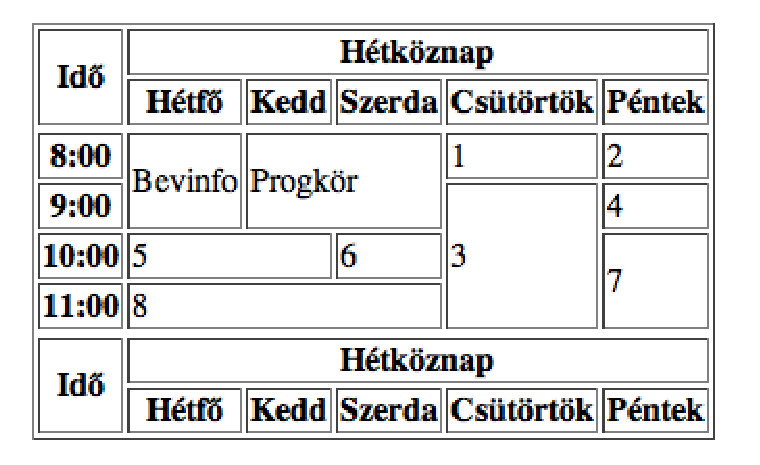
\includegraphics[scale=0.7]{html-table-view.eps}%
\end{center}%
  \caption{Az összetett táblázat (\ref{fig:html-table}.\ ábra) kinézete}%
  \label{fig:html-table-view}%
\end{figure}

A táblázatot a \texttt{table} elem jelöli, a sorokat pedig a \texttt{tr}. Egy
táblázatnak kétfajta cellája lehet, az egyik a fejléchez tartozik, ennek
megfelelően \texttt{th} a neve (table head), a másik az adatok tárolására
szolgál, ez a \texttt{td} (table data). Bár tipikusan az első pár sor a fejléc,
előfordulhat \texttt{th} elem a sorok elején is, akárcsak a láblécben.

Egy cella nem feltétlenül 1x1-es, hiszen nemegyszer össze kell fogni több
oszlopot a fejlécben, vagy éppen sort, ráadásul az adatrészben is
előfordulhatnak. Ha nem adjuk meg, hogy hány sornyi illetve oszlopnyi legyen,
akkor az alapértelmezett 1 értéket kapja, különben legalább az egyiket ki kell
írni. Tehát ha egy $n\times m$-es cellát szeretnénk megadni, ahol $n$ a sorok,
$m$ pedig az oszlopok számát jelöli, akkor azt a \texttt{rowspan} és
\texttt{colspan} attribútumokkal tehetjük meg a következőképpen (az összes nem
1x1-es lehetőséget felsorolva):

\begin{Verbatim}[frame=single]
<td colspan="m" rowspan="n">adat...</td>
<td rowspan="n" colspan="m">adat...</td>
<td rowspan="n">adat...</td>
<td colspan="m"">adat...</td>
\end{Verbatim}

\section{Formázás CSS-sel}\label{sec:html-css}
A \textsc{html}-t egy ideig használták formázásra is, mára azonban szinte csak
\textsc{css} kóddal határozzák meg az oldalak kinézetét. Ez utóbbi nagy előnye,
hogy a stílus (azaz a kinézet) és a tartalom különválik, így akár több
\textsc{html} oldal kinézetét is lehet befolyásolni egyetlen \textsc{css}
állomány módosításával. \Aref{fig:html-css-head}.\ ábrán látható módon lehet a
\textsc{html} dokumentumban megadni a stílust, valamint
\aref{fig:html-css-external}.\ ábrán látható módon lehet akár több külső
\textsc{css} állományt is használni. Természetesen a két megoldás együtt is
használható, például akkor, ha csak az adott oldalhoz kell stílust definiálni
-- bár még ekkor is jobb a külső fájl a könnyebb módosíthatóség és kezelhetőség
miatt.


\begin{figure}[tbh]
\begin{Verbatim}[frame=single]
<!DOCTYPE HTML PUBLIC "-//W3C//DTD HTML 4.0//EN">
<html>
  <head>
  <title>Bach's home page</title>
  <style type="text/css">
    body { 
      font-family: "Gill Sans", sans-serif;
      font-size: 12pt;
      margin: 3em; 
    }
  </style>
  </head>
  <body>
    <h1>Bach's home page</h1>
    <p>Johann Sebastian Bach was a prolific composer.</p>
  </body>
</html>
\end{Verbatim}
\caption{}
\label{fig:html-css-head}
\end{figure}

\begin{figure}[tbh]
\begin{Verbatim}[frame=single]
<!DOCTYPE HTML PUBLIC "-//W3C//DTD HTML 4.0.1//EN">
<html>
  <head>
  <title>Bach's home page</title>
  <style type="text/css">@import "system/default.css";</style>
  <link rel="stylesheet" type="text/css" href="system/tables.css"/>
  </head>
  <body>
    <p>Johann Sebastian Bach was a prolific composer.</p>
  </body>
</html>
\end{Verbatim}
\caption{}
\label{fig:html-css-external}
\end{figure}



Az azonosító lehet egyrészt a fent látható módon egy elem neve,
másrészt egy osztály, harmndrészt pedig egy azonosító. Az első már ismert, így
most tekintsük az utóbbi jettőt. Egy \textsc{html} elem tartozhat valamely
stílusosztályba, amelyet a \texttt{class} attribútum határoz meg, valamint lehet
egy egyedi azonosítója, amelyet a linkeknél említett \texttt{id} attribútum
határoz meg.

A példákban látható módon megadott \textsc{css} definíciókban szereplő azonosító
egy vagy több \textsc{html} elem nevét is tartalmazhatja, pl. \texttt{table.main
  tr.odd td \{...\}}, ami azt jelenti, hogy a \texttt{main} osztályba tartozó
\texttt{table} elemen belül valahol szerepel egy \texttt{odd} osztályú
\texttt{tr} elem, melyben egy \texttt{td} elem található. E \texttt{td} elem
(amely nem feltétlenül létezik, s ekkor a stílusdefiníció nem jut érvényre)
kinézetét befolyásolja. Lényeges, hogy itt nem szülő-gyerek, hanem
szülő-leszármazott (unoka stb.\ ugyanúgy lehet) viszonyról van szó, tehát a
\texttt{table} és \texttt{tr} elem között lehet például egy \texttt{tbody} elem
is, sőt a definíció a \texttt{td} elemben megadott másik táblázatbeli
\texttt{td} elemre is vonatkozik!

A Cascading Style Sheets elnevezés is innen ered, vízesésszerűen vonul végig az
adott beállítás az egyes elemeken. Ha egy általános elemre (pl.\ a
\texttt{td}-re) definiált valami, akkor annak specializált változataira (pl.\
adott stílusosztályba tartozókra: \texttt{td.first}) is vonatkozik az a
beállítás. Természetesen -- a legtöbb esetben -- ez felülbírálható a
specializált esetben is.

Lehet csak az adott \textsc{html} elemre vonatkozó stílusdefiníció, ha a
\texttt{style} attribútumot használjuk, mint például az \textsc{xhtml} 1.0
Transitional változatának \texttt{u} elemének megfelelő, 1.0 Strict és 1.1-es
változatában használható megoldás: \texttt{style="text-decoration: underline"}.

% Local Variables:
% fill-column: 80
% mode: latex
% End:

  \chapter{A Linux}%
\label{cha:linux}

A Linux egy Unix-szerű operációs rendszer (OS), vagyis sok mindenben hasonlít
mind a használat, mind a programozás tekintetében. E fejezet az eredetét és az
alapvető működését írja le.


\section{A Linux eredete}

A Linuxot alapvetően nagy tudású hackerek készítik, azonban bárki hozzájárulhat
jobbá tételének. A (mai) hackereknek saját kultúrájuk van, amelynek története az
1960-as évekig nyúlnak vissza ekkor kapott ugyanis az \textsc{mit}
(Massachusetts Institute of Technology) vasútmodellező köre egy
\textsc{pdp-1}-es gépet, \cite{bazar,bazar-web}, amelyhez programozási
eszközöket, nyelvet, sőt, teljes kultúrát alakíttak ki. Ebből jött létre az
egyetem mesterséges intelligencia laborja, amely a 80-as évek vezető
MI-központja volt.

A következő jelentős mérföldkő az ARPAnet kialakításának éve, 1969 volt. E
hálózat eredetileg katonai célokra szolgált, tesztkörnyezetként (amelynek háború
esetén is működnie kellett), mely egész földrészeken átívelt, idővel azonban
rácsatlakoztak az egyetemek is. Az információ most már messzebbre eljuthatott,
ezáltal az \textsc{mit}-beli kutatóközpont hatása is megnőtt.

A \textsc{pdp} sorozat 10-es számú gépe '67-től 15 éven keresztül meghatározó
volt, és bár készült hozzá operációs rendszer is, az MIT hackerei saját
változhatot készítettek, amely az \textsc{its} (Incompatible Time-Sharing System,
Inkompatibilis Időosztásos Rendszer) nevet kapta, számos újítást
tartalmazott. És valóban jól működött. Alapvetően assemblyben íródott, tehát a
kód csak ezen a gépen volt futtatható. Nemegy program \texttt{lisp}-ben íródott,
a legismertebb a ma is használatos \textsc{emacs} programszerkesztő.


Szintén '69-hez kötődik egy másik esemény is. Ken Thompson, a Bell-Laps egyik
hackere megalkotta a Unixot. Eredetileg a Multics nevű OS fejlesztésén
dolgozott, amelyen olyan újításokkal kísérletezett, amelyek elfednék az
operációs rendszer bonyolultságát a felhasználók elől. A rendszer azonban
kezdett túl bonyolulttá válni, így a Bell Labs elállt a piacra dobásától. Ennek
nyomán Thompson nekiállt egy újabb rendszer írni az eddigi ötletei
alapján. Ebben nyújtott segítésget Dennis Rithcie, aki egy új nyelvet dolgozott
ki a kezdeti Unix rendszr számára, a C-t.

Míg eddig minden OS assembly-ben íródott, a Unix már nem, ugyanis már nem volt
fontos a kód adott hardverre történő optimalizálása, s az akkori
fordítóprogramok mellett egy teljes operációs rendszer is megírhatóvá vált egy
magasabb szintű nyelven, például C-ben is.

A C gépfüggetlen volt, így 1978-ra számos géptípusra sikerült átültetni a
Unixot. A nyelv is egyszerű, könnyen fejben tartható volt sok egyéb nyelvtől
eltérően.

A Unix még egy előnnyel rendselkezett: beépítetten tartalmazta az
\texttt{uucp}-t, amely kis sebesságű, megbízhatatlan kapcsolatot tett lehetővé
telefonvonal felhasználásával.

A '80-as évek elején Richard R. Stallman -- akit bejelentkezési azonosítójáról
`rms'-ként is ismerhetünk -- megalapította a Free Software Foundation-t
(\textsc{fsf}-t). A Unix már grafikus felületet is adott, az X Window System-et,
amelyet gyakran csak X-nek nevezünk. A '90-es évek ben az olcsó, nagy
teljesítményű számítógépek terjedtek el.

Bár a hardver fejlődött, nem volt hozzá olcsó szoftver, ezért az
\textsc{fsf}-nél egy Unix rendszermag (\emph{kernel}), a \textsc{hurd}
fejlesztésébe kezdtek, amely azonban nem folytatódott, egészen 1996-ig állt.

Az \textsc{fsf} azonban adott mást: tömérdek ingyenes, nyílt forráskódú
programot, amelyeket \textsc{gnu} programoknak neveztek el. A \textsc{gnu} egy
betűszó, a `\textsc{GNU} is Not Unix' rövidítése. A be nem fejezett
rendszermaggal együtt a \textsc{gnu/hurd} elnevezést kapta.

Ezekkel az eszközökkel állt neki egy finn egyetemista -- Linus Torvalds -- egy
rendszermag elkészítésének. 1991 nyarára sikerült egy működő
lemezmeghajtó-vezérlő kódot írnia. E kernel a Linux nevet kapta, és a
felhasználói programokkal együtt gyakran  GNU/Linux-nak nevezik, bár ez ma már
nem pontos, hiszen számtalan nem \texttt{gnu} program is van rajta.

Ugyancsak ezekben az időkben portolták az egyik Unix változatot, a
\textsc{bsd}-t -- melyet a Berkeley egyetemen készítettek, és a név a Berkeley
Software Distribution rövidítése -- 386-os gépekre.

A Linuxot igazán sikereressé az Internet és a világháló elterjedése tette.

\section{A fájlrendszer}
A Linux fájlrendszer egyetlen, összefüggő fából áll, a merevlemez különböző
partícióit ennek a fának valamely csúcsára lehet rácsatolni, feltéve ha az adott
csúcs egy könyvtár. Néhány esetben még az is elvárás, hogy a könyvtár üres
legyen. 

A File System Hierarcy Standard\acite{fhs} (\textsc{fhs}) tartalmazza, hogy mely
könyvtáraknak mi a szerepük, ezek közül sok opcionálos, vagy csupán a régebbi
rendszerekkel való kompatibilitást hivatott biztosítani. néhány példát
\aref{tab:linux-fs}.\ táblázatban láthatunk.


\begin{table}%
\center%
\begin{tabular}{@{}ll@{}}\toprule
Könyvtár & Funkció\\\midrule
/boot & A Linux kernelét tartalmazza, induláskor használt\\
/bin  & A rendszer indulásakor is használt programok\\
/dev  & Eszközfájlok a hardverek kezeléséhez\\
/root & A root felhasználó home könyvtára\\
/sbin & Rendszerinduláskor is használt programok a root számára\\
/usr  & A felhasználói programok és azok adatai\\
/usr/bin & Mindenki számára elérhető programok, melyek\\
& nem szükségesek a rendszer elindulásakor
\\\bottomrule
\end{tabular}
  \caption{Néhány könyvtár és azok funkciója}
  \label{tab:linux-fs}
\end{table}

%\section{A Linux rendszer elindulása}


%\section{A legfontosabb beállítások}


%\section{Használat}

% Local Variables:
% fill-column: 80
% mode: latex
% End:

  \chapter{A parancsértelmező használata}%
\label{cha:shell}


A parancsértelmező a Unixos időszakból származik, azóta számtalan eltérő tudású
verziója jelent meg. Erre példa a \texttt{tcsh}, \texttt{ksh}, \texttt{bash},
\texttt{sh}. Ma ez utóbbin egy \textsc{posix} szabványban \cite{posix:shell}
rögzített tulajndoságokkal rendelkező változatot értjük, azonban előfordulhat,
hogy többet tud, például akkor, ha csupán egy symlink a \texttt{bash}-re.

A jegyzet hátralévő része a bash-ről szól. A bash a Bourne Again SHell
rövidítése.

A Linux rendszereken a bash az alapértelmezett parancsértelmező, ezért fontos,
hogy tisztában legyünk a működésével. E fejezet nagy vonalakban vázolja a
lehetőségeket, a későbbiekben pedig kitérünk az egyes részletekre,
kategóriánként csoportosítva. Mivel a bash önmagában csupán korlátozottan
használható, ezért kezdettől fogva fontos szerep jut a rendszer további,
bash-ből használható programjainak is.

\section{A bash alapjai}

Amikor karakteres felületen vagy éppen ssh-n keresztül jelentkezünk, akkor a
bash indul el, és várja, hogy parancsokat gépeljünk be számára. Bár a grafikus
felületen nem találkozunk vele, egy terminált megnyitva (amilyen az
\texttt{xterm}, vagy a \texttt{Konsole}) szintén e parancsértelmezőt indítjuk
el.

Ha már fut, akkor többféleképpen léphetünk ki belőle. az egyik lehetőség a
Ctrl-D leütése, amellyel jelezzük, hogy nem kívánunk további parancsokat kiadni,
vagyis a bemenete végetért. A másik az \texttt{exit} parancs -- utasítás --
begépelése, amely után enter-t ütve a bash befejezei futását. Ha nem indítottunk
el másik programot, mely lehet akár egy másik bash példány is, akkor a rendszer
kiléptet minket az ssh esetén, vagy pedig bezáródik a terminál ablaka.

A Ctrl-D a legtöbb program számára azt jelenti, hogy véget ért a bemenete,
vagyis a billentyűzetről nem fog újabb sorokat kapni, ám ezzel a bash esetén a
rendszerből is ki is lehet jelentkezni, ami lehet nem szándékos is, ezért a
\aref{cha:env-vars}.\ fejezetben látni fogjuk, hogyan lehet ezt elkerülni.

A futó parancsértelmező vár valamilyen bemenetre, amit értelmezni tud, majd
pedig lefuttatni, a parancs végét általában az enter billentyű leütésével
jelezhetjük -- ám van olyan parancs is, amely a későbbi sorokban folytatódik.
A hibásan beírt parancsot könnyen
javíthatjuk, mivel elegendő a kurzormozgató billentyűkkel balra-jobbra
navigálni, és beszúrni az új, már jó kódot, a régit pedig törölni. A korábban
kiadott parancsok is elérhetőek a fel-le gombokkal lépegetve közöttük. Sőt, az
eddig kiadott -- és megjegyzett -- parancsokat meg is tekinthetjük a
\texttt{history} parancs kiadásával. Egy korábban kiadott parancsot úgy is
megtalálhatunk, ha a C-r (control és r) billentyűk leütése után beírjuk a
parancs egy részletét.

\section{Parancsok általában}

A legtöbb parancs a következő formában működik:

\begin{VerbExample}
program opciók paraméterek
\end{VerbExample}

Ebből egyedül a \texttt{program} kötelező, a többi nem. Az opciók mínuszjellel
kezdődnek és egy karakter hosszúak, melyekangol ábécé kis- és nagybetűi, valamint
számjegyek lehetnek. Ez a régi Unixokon elterjedt verzió, ahol még fontos volt,
hogy minden minél rövidebben leírható -- begépelhető -- legyen. Ma már sokszor
az olvashatóság fontosabb, illetve egyes opcióknak nincs is egy karakteres
változata, ezek angol elnevezése ``long options'', hoyyszú opciók. Mindegyik két
darab mínuszjellel kezdődik, majd pedig legalább egy szó áll ott, több szó
esetén köztük mínuszjel áll. 

Erre példa a \texttt{wc} szűrő, amelynek az itt látható opciója a leghosszabb
beolvasott sor hosszát adja meg:

\begin{VerbExample}
wc -L
wc --max-line-length
\end{VerbExample} 

Egyes programok megengedik azt, hogy az opciók a paraméterek után legyenek.

Akár megengedik, akár nem, fontos, hogy meg lehessen őket különböztetni
egymástól, ezért a mínuszjellel kezdődő paraméter (például fájlnév) esetén e
határt valahogy jelölni kell.

Fájlnév esetén ez még egyszerű, hiszen a probléma megkerülhető az aktuális
könyvtár explicit használatával: ``./-file'', a gond akkor van, ha a paraméter
nem fájlnév. Erre egy speciális opció van, a mínuszjel: ``--''. Például az
összes fájl vagy könyvtár tulajdonságainak listázása -- lásd később:

\begin{VerbExample}
 ls -l -- *
\end{VerbExample}

Ez esetben az opció önállóan áll, ám a legtöbb opció összevonható, például:

\begin{VerbExample}
ls -l -A -R
ls -lAR
head -q -n 8
head -q -n8
head -qn8
\end{VerbExample} 

\subsection{Segítség a használható parancsokhoz}

Az összes programot nem lehet és nem is szükséges fejben tartanunk, ugyanis
számos lehetőséget nyújt egy Linux rendszer az információk megszerzésére. Ha
ismerjük a programot, akkor annak leírását, kézikönyvlapját a \texttt{man}
paranccsal kaphatjuk meg, vagy pedig az \texttt{info} paranccsal. Ha nem
ismerjük a parancs nevét, de tudjuk, mit csinál, akkor az \texttt{apropos}
paranccsal találhatjuk meg (ez egyébként ugyanaz, mint a \texttt{man
  -k}). Mindegyik esetben a keresendő program nevét paraméterben kell megadni,
esetleg a fejezetet is, ugyanis a kézikönyvlapok fejezetekbe tartoznak, és több
fejezetben is lehet azonos parancs.

A következőkben a kiadható parancsokra láthatunk példákat, mindegyiket egy-egy
rövid leírás követi a bash által értelmezett megjegyzés formájában, amely a
kereszt (hash mark, '\#') jeltől kezdve a sor végéig tart.

\begin{Verbatim}[xleftmargin=10mm]
man bash       # a bash kézikönyvlapja - nagyon hosszú
apropos copy   # mivel is tudunk másolni?
info coreutils # néhány alapvető parancs leírása
man 5 fstab    # a  /etc/fstab leírása az 5. fejezetben
\end{Verbatim}



\section{Ismerkedés a rendszerrel}

Az előző fejezetben már láthattuk, hogy hogyan néz ki a Linux fájlrendszere,
most megismerkedünk az ezen dolgozó parancsokkal, valamint néhány további
hasznos eszközzel.

\subsection{Fájlok, könyvtárak}

Az adataink egyetlen könyvtárban és annak alkönyvtáraiban találhatóak, ezt
nevezzük home könyvtárnak (home directory). Néhány rendszeren például a
honlapokat mégis egy másik helyen tároljuk, így valójában több helyen is
lehetnek a fájljaink, de nem tekinthető szokásosnak.

E könyvtárba a \texttt{cd} paranccsal léphetünk, egy másikba pedig hasonlóan,
csak meg is kell adnunk a könyvtár nevét:
\begin{VerbExample}[commandchars=\\\{\}]
cd \textit{könyvtárnév}
\end{VerbExample}
Azt, hogy hol állunk, a \texttt{pwd} paranccsal kérdezhetjük le, például:

\begin{VerbExample}
~ > pwd
/home/panther
\end{VerbExample}

A parancsot a \emph{prompt} után írhatjuk be, amelynek a végét általában egy
dollárjel (\$) szokta jelezni. A promptot néhol készenléti jelnek is nevezik. A
bash esetén szabadon módosítható a tartalma, ezért előfordulhat, hogy az
aktuális könyvtár nevét is tartalmazza, például Gentoo linuxok esetén a home
könyvtár nevét a `~' karakter (tilde, hullámvonal) helyettesíti:

\begin{VerbExample}
panther@tassadar ~/git/panther-elte/progkor/doc $ cd
panther@tassadar ~ $
\end{VerbExample}

Könyvtár létrehozására illetve törlésére az \texttt{mkdir} és \texttt{rmdir}
parancsok szolgálnak, mindegyik egy vagy több könyvtár nevét várja. Fájlok
törlésére pedig az \texttt{rm} parancs való:

\begin{VerbExample}
mkdir a a/b almafa  # ezen könyvtárak létrehozása
rmdir almafa        # egyből töröljük is
rm -r a             # az rm könyvtárat is töröl
\end{VerbExample}

A példákban az \texttt{rmdir} csupán üres alkönyvtárat tud törölni, ámde az
\texttt{a} könyvtár nem volt az, így kényelmesebb volt az \texttt{rm} parancsot
használni, ami az \texttt{a} tartalmát is törli a \texttt{-r} opció hatására. Ez
utóbbi jelentése rekurzív törlés: előbb a fájlokat, majd pedig az így üressé
vált könyvtárakat törli.

Fájlokat tipikusan egy \emph{editorral} (kisebb-nagyobb tudású
``szövegszerkesztő'' programmal) hozunk létre, vagy pedig másolással. Az
előbbiről \aref{sec:editors}.\ alfejezet foglalkozik. Az utóbbit a \texttt{cp}
paranccsal tehetjük meg, illetve ha áthelyezni, mozgatni szeretnénk, akkor pedig
az \texttt{mv} parancsot használhatjuk.

\begin{VerbExampleNum}
cp a b             # 1 fájl másolása
cp a b c/          # több fájl másolása
cp -r könyvtár  b  # könyvtár másolása
cp -ar könyvtár b  # ... jogok megőrzése
mv a b             # átnevezés/áthelyezés
mv -i a b          # interaktív
\end{VerbExampleNum}

E példákban az opcióknak nagy szerepük van. A \texttt{cp} önmagában csak fájlt
tud másolni, könyvtárat csupán a \texttt{-r} opcióval együtt a 3.\ példa
szerint. Ha több fájlt vagy könyvtárat másolunk, akkor az utolsó kötelezően
könyvtár, ebben lesz az új tartalom. A 4.\ példában a \texttt{-a} opció
garantálja, hogy a fájlok tulajdonságai sem változnak (tulajdonos, módosítási
idő és jogosultság). Az \texttt{mv} parancsnak nem szükséges megadnunk a
\texttt{-r} opciót -- nincs is ilyen --, ettől eltekintve ugyanaz igaz rá, mint
a \texttt{cp}-re. A 6.\ példában a \texttt{-i} opció hatására az \texttt{mv}
rákérdez minden egyes fájl esetén, ha a célfájl már létezik, vagyis a véletlen
felülírástól véd. Ez használható a \texttt{cp} és az \texttt{rm} parancsokkal
is, utóbbinál a véletlen törlés lehetőségét zárja ki.


\subsection{Környezet - más felhasználók}

A Unix rendszereken megszokott, hogy többen is használják egyszerre, tehát ha
egy szerverre ssh-n keresztül bejelentkezünk, akkor nagy valószínűséggel lesz
más felhasználó is. Próbaképpen nézzünk is szét:

\begin{VerbExample}
panther@panda:~$ users
dojo panther panther sz sz sz
panther@panda:~$ who
dojo     pts/1        Jan 27 09:53 (53d82d1e.adsl.enternet.hu)
sz       pts/3        Jan 27 11:47 (ia8vb9l7ul.adsl.datanet.hu)
sz       pts/4        Jan 27 11:49 (ia8vb9l7ul.adsl.datanet.hu)
panther  pts/5        Jan 27 11:51 (valerie.inf.elte.hu)
sz       pts/6        Jan 27 11:51 (ia8vb9l7ul.adsl.datanet.hu)
panther  pts/7        Jan 27 11:53 (dsl54008339.pool.t-online.hu)
panther@panda:~$ w
 11:53:25 up 9 days, 19:54,  6 users,  load average: 0.02, 0.01, 0.00
USER     TTY      FROM              LOGIN@   IDLE   JCPU   PCPU WHAT
panther@panda:~$ uptime
 11:53:28 up 9 days, 19:54,  6 users,  load average: 0.02, 0.01, 0.00
\end{VerbExample}

Ezen parancsok sokféle információt tartalmaznak, tekintsük sorban. A legelső a
\texttt{users} volt, amely a bejelentkezett felhasználók neveit írja ki. Ha
valakinek az azonosítója egynél többször szerepel, akkor ugyanennyiszer
jelentkezett be. A következő a who, amely a felhasználók azonosítóját, az
általuk használt terminált (a \texttt{/dev} alatti fájl nevét), a bejelentkezés
idejét, valamint azon gép nevét listázza, ahonnan bejelentkezett. A \texttt{w}
első sora az \texttt{uptime} parancs kimenetét tartalmazza, a többi pedig
további adatokat közöl a bejelentkezett felhasználókról. Ha grsecurity
\cite{grsecurity}, valamint pax \cite{pax} kiegészítésekkel biztonságosabbá tett
rendszeren adjuk ki, akkor gyakran üres a lista. Egy otthoni gépen viszont már
többet láthatunk:

\begin{VerbExample}
panther@tassadar ~ $ users
panther panther
panther@tassadar ~ $ who
panther  :0           2008-01-27 09:52
panther  pts/7        2008-01-27 11:59 (artanis.panthernet)
panther@tassadar ~ $ w
 11:59:09 up  2:08,  2 users,  load average: 0,16, 0,14, 0,13
USER     TTY        LOGIN@   IDLE   JCPU   PCPU WHAT
panther  :0        09:52   ?xdm?   5:43   0.00s /bin/sh /usr/kde/3.5/bin/startkde
panther  pts/7     11:59    7.00s  0.16s  0.16s -bash
panther@tassadar ~ $ uptime
 11:59:12 up  2:08,  2 users,  load average: 0.16, 0.14, 0.13
\end{VerbExample}

A \texttt{:0} azt jelzi, hogy az adott felhasználó grafikus felületen
jelentkezett be, a nullás azonosítójú képernyőn -- több grafikus felület is
futhatna egyszerre. A ``LOGIN@'' a bejelentkezési időt adja meg, az ``IDLE'' azt
az időt, amennyi ideje inaktív. Grafikus felület esetén ilyen nincsen, ám ssh
esetén már van, ez látszik is a példában, 7 másodperce inaktív a felhasználó --
csak a példa kedvéért bejelentkeztem egy másik gépről. A JCPU és a PCPU a
felhasznált processzoridőt adja meg, a WHAT pedig a futtatott
programot. Természetesen nincsen olyan, hogy \texttt{-bash}, a mínusz jelnek
jelen esetben speciális jelentése van, méghozzá az, hogy interkatív vagyis
bejelentkezési shellről van szó, ahova a felhasználó gépelhet.

Az \texttt{uptime} kimenete sokszor érdekesebb, az első része a pontos időt írja
ki, majd az ``up'' szó után a futási időt, például 2 óra 8 perce megy a gép,
vagy éppen a panda esetén 9 napja, 19 órája és 54 perce, továbbá 2 illetve 6
bejelentkezett felhasználó van. A ``load average'' az átlagos terhelés az elmúlt
egy, öt, valamint 15 percben, vagyis átlagosan hány folyamat (futó program)
kívánta használni a processzorokat. Amíg ezek az értékek legfeljebb akkorák,
mint ahány processzor -- pontosabban processzormag -- van a gépben, addig
nincsen gond, utána viszont már túlterhelt. Ez előfordulhat akkor, ha valamelyik
program hibásan működik, vagy túl sokan használják a gépet, de lehet
természetesnek nevezhető állapot is, amikor átmenetileg nagy számításigényű
feladatot hajt végre valamely program.

Az egyes felhasználókról további információkat is megtudhatunk a finger parancs
kiadásával:

\begin{VerbExample}
panther@tassadar ~ $ finger
Login    Name                   Tty      Idle  Login Time   Office     Office Phone
panther  Tóth László Attila *:0             Jan 27 09:52
panther  Tóth László Attila  pts/7      13  Jan 27 11:59 (artanis.panthernet)
panther@tassadar ~ $ finger -m panther
Login: panther                          Name: Tóth László Attila
Directory: /home/panther                Shell: /bin/bash
On since Sun Jan 27 09:52 (CET) on :0 (messages off)
On since Sun Jan 27 11:59 (CET) on pts/7 from artanis.panthernet
   14 minutes 12 seconds idle
New mail received Wed Jan 23 21:52 2008 (CET)
     Unread since Sat Jan  5 15:30 2008 (CET)
No Plan.
\end{VerbExample}

Paraméterek nélkül kiadva a bejelentkezettt felhasználók nevét is kiírja. A
következő példában a \texttt{-m} opció nélkül nem csak a felhasználónevet
keresné, hanem a valódi névben is megnézné, hogy az adott karakterosozat
szerepel-e, így további felhasználókat is listázna, így viszont a pontos
illeszkedést kapjuk. A listázott adatok: azonosító (login), név, home könyvtár,
parancsértelmező (shell), mikor, melyik terminálon és honnan jelentkezett be. A
``messages off'' azt jelenti, hogy nem fogad el üzeneteket, ugyanezt jelenti az
első példában a ``TTY'' oszlopban látható csillag karakter is.

Kiírja, hogy van-e levele, és a \texttt{.plan} fájl tartalmát is, feltéve, ha el
tudja olvasni. Nálam nincsen ilyen fájl, ezért a ``No plan'' szöveg jelenik meg.

Az üzenetek tiltását és engedélyezését a \texttt{mesg} paranccsal lehet
szabályozni, a \texttt{y} paraméterrel engedélyezni, \texttt{n}-nel pedig
tiltani:

\begin{VerbExample}
mesg y              # engedélyezés
mesg n              # tiltás
\end{VerbExample}


Hogyan tudunk egy másik felhasználónak írni? A Unix világban már nagyon
hosszúnak számító \texttt{write} paranccsal. Hosszú, ugyanis általában két,
esetleg három karakteres a legtöbb parancs. Paramétere annak a felhasználónak az
azonosítója, akinek gépelni szeretnénk. Mivel a program a terminálra ír,
miközben a másik rajta dolgozik, ezért úgy illik, hogy valahogyan jelezzük,
mikor fejeztük be azt, amit épp írunk, és ekkor a másik elkezdhet írni. Enélkül
a másik félig elkezdett sorában fog megjelenni az üzenetünk, ami nagyon zavaró.
\ut{write valaki}
A programból a Ctrl-D leütésével léphetünk ki.

\subsection{Környezet - a számítógép}

Fentebb láthattuk, hogyan lehet megtudni, mennyi ideje megy a számítógép, és
mekkora a terhelése. Erre szolgált az \texttt{uptime} parancs. Azonban további
információkat is meg lehet tudni, így a \texttt{df} az egyes partíciók
összméretét, foglalt és szabad részének méretét írja ki:

\begin{VerbExample}
panther@tassadar ~ $ df
Fájlrendszer          1K-blokk   Foglalt    Szabad Fo.% Csatl. pont
/dev/sda3            194396620 167506840  26889780  87% /
udev                     10240       224     10016   3% /dev
shm                    2023320         0   2023320   0% /dev/shm
panther@tassadar ~ $ df  -h
Fájlrendszer         Méret  Fogl. Szab. Fo.% Csatl. pont
/dev/sda3             186G  160G   26G  87% /
udev                   10M  224K  9,8M   3% /dev
shm                   2,0G     0  2,0G   0% /dev/shm
panther@tassadar ~ $ df  --si
Fájlrendszer          Méret  Fogl.  Szab.  Fo.% Csatl. pont
/dev/sda3              200G   172G    28G  87% /
udev                    11M   230k    11M   3% /dev
shm                    2,1G      0   2,1G   0% /dev/shm
panther@tassadar ~ $ df  -m
Fájlrendszer          1M-blokk   Foglalt    Szabad Fo.% Csatl. pont
/dev/sda3               189841    163581     26260  87% /
udev                        10         1        10   3% /dev
shm                       1976         0      1976   0% /dev/shm
\end{VerbExample}

Általában ezekkel az opciókkal érdemes használni, alapesetben 1024 bájtos
blokkal számol. A \texttt{-h} hatására jól olvasható módon írja ki, továbbra is
1024-es szorzóval (K = kiB, M = MiB, G=GiB stb.). A \texttt{--si} ugyanez, ezres
szorzóval (vagyis itt a K kB-ot jelent stb.), a \texttt{-m} pedig MiB-ban adja
meg a méretet.

A rendelkezésre álló memóriát is megkaphatjuk a \texttt{free} segítségével,
opciók nélkül 1 kiB-os blokkok számában, \texttt{-m} esetén pedig MiB-ban.

\begin{VerbExample}
panther@panda:~$ free
             total       used       free     shared    buffers     cached
Mem:        246176     195508      50668          0          0      83092
-/+ buffers/cache:     112416     133760
Swap:       506008       3016     502992
panther@panda:~$ free -m
             total       used       free     shared    buffers     cached
Mem:           240        190         49          0          0         81
-/+ buffers/cache:        109        130
Swap:          494          2        491
\end{VerbExample}

Végezetül magának a hardvernek az adatait is megtekinthetjük a
\texttt{/proc/cpuinfo} fájl listázásával és az \texttt{lspci} használatával. A
példában szereplő lista nem teljes és a sorok végét sem tartalmazza.

\begin{VerbExample}
panther@panda:~$ cat /proc/cpuinfo
processor       : 0
vendor_id       : GenuineIntel
cpu family      : 6
model           : 8
model name      : Celeron (Coppermine)
stepping        : 10
cpu MHz         : 906.741
cache size      : 128 KB
fdiv_bug        : no
hlt_bug         : no
f00f_bug        : no
coma_bug        : no
fpu             : yes
fpu_exception   : yes
cpuid level     : 2
wp              : yes
flags           : fpu vme de pse tsc msr pae mce cx8
bogomips        : 1816.05

panther@panda:~$ lspci
00:00.0 Host bridge: VIA Technologies, Inc. VT82C693A/694x [Apollo PRO 
00:01.0 PCI bridge: VIA Technologies, Inc. VT82C598/694x [Apollo MVP3/
00:07.0 ISA bridge: VIA Technologies, Inc. VT82C686 [Apollo Super South]
\end{VerbExample}

\section{Editorok}%
\label{sec:editors}

Amikor egy-egy szövegfájlt, szkriptet vagy éppen valamely program egyik
forrásfájlját módosítjuk, akkor hasznos, ha a használt
\emph{editor} elég nagy tudású ahhoz, hogy támogassa munkánkat. Egy rendszeren
ebből sokféle van, a legminimálisabb tudásútól (\emph{mcedit}, \emph{pico})
a legtöbbet tudóig (\emph{ViM}, \emph{Emacs}). Az előbbit illik ismerni, hiszen
lényegében bármely Unix változat elé ülünk le, vagy ez, vagy pedig ennek az őse,
a \emph{vi} biztosan fenn lesz az adott gépen.

\subsection{A vim}

A vim alapvetően két módban futhat, az egyikben parancsokkal lehet vezérelni, a
másikban pedig a szöveget módosítani. A váltás közöttük például az \texttt{ins}
és az \texttt{esc} billentyűk használatával lehetséges.

A ``parancsmód'' főbb lehetőségeit \aref{tab:vim-ex}.\ táblázat foglalja össze.

\begin{table}\center%
\begin{tabular}{ll}\toprule
Billentyű & Jelentés\\\midrule
:q & kilépés\\
:q!& kilépés mentés nélkül\\
:w & mentés\\
:syntax on & syntax highlight -- kódszínezés\\
:!parancs & parancs futtatása a shellben\\
v & kijelölés\\
shift-v & sorok kijelölése\\
\bottomrule
\end{tabular}
  \caption{A vim néhány billentyűkombinációja}
  \label{tab:vim-ex}
\end{table}


\subsection{Az emacs}

Az Emacs (helyesen kiejtve kb.\ imeksz) egy több évtizedes múlttal rendelkező
editor, hiszen lisp-ben íródott. Magát a programot kevesen fejlesztik, ám
\emph{lisp} nyelven bárki által programozható, és számtalan kiegészítés létezik
hozzá. A vi-hoz hasonlóan szokatlan a működése, mert bár nincs megkülönböztetve,
hogy mikor lehet parancsot kiadni, s mikor lehet szöveget szerkeszteni, a
vezérlése billentyű-kombináció sorozat révén lehetséges. Ezek megértéséhez
tudnunk kell, hogy a Control gombot C-vel, a Meta gombot pedig M-mel
rövidíti. Ez utóbbi \textsc{pc}-k esetén az Alt gomb, míg Mac esetén a
Command. Például C-x C-s a mentés.

\begin{table}\center
\begin{tabular}{ll}\bottomrule
Billentyű-kombináció &Jelentés\\\midrule
C-x C-c & kilépés\\
C-x C-s & mentés\\
C-x C-f & másik fájl megnyitása a név megadásával\\
C-x C-w & mentés másik név megadásával\\
C-SPACE & kijelölés kezdete\\
C-x w   & kivágás\\
C-x y   & beillesztés\\\midrule
C-x b   & ugrás másik fájlra (pufferre)\\
C-x 1   & 1 részre osztott ablak\\
C-x 2   & vízszintesen tagolt ablak\\
C-x 3   & függőlegesen tagolt ablak\\
\bottomrule
\end{tabular}
  \caption{Emacs vezérlése}
  \label{table:emacs}
\end{table}



\section{Néhány példa}

A bash működése viszonylag egyszerű, ám összetett, bonyolult programok --
szkriptek -- is viszonylag könnyedén írhatóak segítségével is, melyek elsősorban
szövegfeldolgozásra, vagy pedig gyakran ismétlődő tevékenység elvégzésére
szolgálnak.

A következő példa azt mutatja meg, hogy egyszerű eszközöket felhasználva egy
bonyolultabb erdményt is megkaphatunk:

\begin{VerbExampleNum}
panther@panda:~$ cat /proc/cpuinfo | grep cpu\ MHz
cpu MHz         : 906.741
panther@panda:~$ grep cpu\ MHz /proc/cpuinfo | cut -f2 -d:
 906.741
\end{VerbExampleNum}

Az első parancsban a \texttt{cat} immár ismerős, ennek kimenetét módosítja a
\texttt{grep}, a mögötte álló szöveget ('cpu MHz') tartalmazó sorokat hagyja
csak meg, azaz megszűri. Innen kapták a \texttt{grep}-hez hasonló programok a
\emph{szűrő} elnevezést, hiszen a bemenetüket megszűrik vagy
átalakítják. Majdnem mindegyik elfogad fájlneveket is, ezért a \texttt{cat}
paranccsal nem is szükséges kiiratnunk a tartalmukat, hogy e kimenetet
használjuk fel egy másik program bemeneteként. Ez utóbbi esetben a két parancs
egy \emph{csővezezetéket} -- angolul: pipe -- alkot, és a köztük álló
karakternek is ez a neve (és magyar billentyűzet-kiosztás esetén egy
\textsc{pc}-n az AltGr-W ``billentyű-kombináció'' csalja elő). A \texttt{cut} a
második mezőt hagyja csak meg ebben a példában, a mezőelválasztó karakter pedig
a kettőspont volt.

Az összes ``.txt'' végződésű fájl nevének kiírássára is számos lehetőség van,
például:

\begin{VerbExampleNum}
~ $ ls *.txt
a.txt b.txt
~ $ ls -1 *.txt
a.txt
b.txt
~ $ find . -name '*.txt'
./a.txt
./b.txt
~ $ for i in *.txt; do echo $i; done
a.txt
b.txt
~ $ find . -iname '*.txt'
a.txt
a.TXT
b.txt
\end{VerbExampleNum}

Az első két parancs esetén a ``*.txt'' önmagában, idézőjel vagy aposztróf nélkül
áll, ekkor a bash behelyettesíti az ott álló fájlneveket, tehát az első parancs
azonos az

\begin{VerbExample}
ls a.txt b.txt
\end{VerbExample}

\noindent kiadásával, amikor listázzuk e fájlokat. További tulajdonságokat az
\texttt{ls -l} paranccsal lehet megtekinteni, az \texttt{-l} opció esetén a
jogosultságokat, tulajdonost, csoportot és módosítási időt is láthatjuk. A
második példában a \texttt{-1} opció hatására minden fájlnév külön sorba kerül.

Az ötödik sorban a \texttt{find} az aktuális könyvtárban -- melynek jele az egy
pont -- és annak alkönyvtáraiban keresi az összes \texttt{.txt} végződésű fájlt
és könyvtárat. Ekkor a ``*.txt'' aposztrófok között áll, ezért a program
változtatás nélkül, ebben a formában kapja meg. A 12.\ sorban lévő változat a
\texttt{-iname} paramétert használja, ekkor a fájlnévben lévő kis-és nagybetűk
közt nem tesz különbséget, bár a Linux alapvetően megkülönbözteti a kis- és
nagybetűket.

A 9.\ sorban lévő for utasítás (ciklus) ugyanazt írja ki, mint az \texttt{ls
  -1}, csak bonyolultabb az alakja, amely más feladatoknál lényeges. Az
\texttt{i} egy változónév, amely ekkortól létezik, és a \texttt{\$i} formában
kapjuk meg az értékét. Az \texttt{in} után egy lista szerepel, amely minden
elemének értékét egyszer felveszi az \texttt{i} változó. Mint fentebb láthattuk,
a bash itt is kifejti a \texttt{*.txt} kifejezést, vagyis az \texttt{in a.txt
  b.txt} az, ami ténylegesen le is fut. A cklus magja a \texttt{do} és
\texttt{done} kulcsszavak között szerepel.

A fenti parancsok között van még egy lényeges különbség: a \texttt{find} esetén
aposztrófok között szereplő ``*.txt'' biztosan működik, míg nagyon sok fájl
esetén az összes többi nem, ugyanis ekkor nem fér el a parancssorban, egy
utasítás hossza fájlnévvel, mindennel együtt nagyjából 16 KiB méretű lehet.

\section{Szkriptek}
\label{sec:scripts}

Egy szkriptfájl egy olyan szöveges állomány, amely valamely program által
értelmezhető utasításokat -- parancsokat -- tartalmaz. Ahhoz, hogy ezt
programként használhassuk, futtathatóvá kell tenni. Amely program képes egy
parancsokat tartalmazó fájlt feldolgozni, ahhoz írható szkriptfájl
(parancsfájl). 

Valójában a kettő nem teljesen ugyanaz, mivel a parancsokat tartalmazó állományt
paraméterként megadjuk az adott programnak, míg a szkriptfájlt le is tudjuk
futtatni, anélkül, hogy lényeges lenne, mely program dolgozza fel. A bash is
ilyen program, valamint a sed is, -- ez utóbbi alapvetően szöveghelyettesítésre
szolgál és róla bővebben \aref{cha:szűrők}.\ fejezetben lesz szó, -- amely a
\texttt{-f} opció után vár egy fájlnevet. 

Mi a bash-t használjuk parancsértelmezőnek, így felmerül a kérdés, hogy a bash
honnan tudja, melyik programhoz tartozik a szkript?  A legelső sor határozza
meg, hogy melyik parancs fogja lefuttatni, melynek a szerkezete:
\texttt{\#!programnév}, vagy ha további opciók szükségesek, akkor
\texttt{\#!programnév opciók}. Ez a bash esetén \texttt{\#!/bin/bash}, a sed
esetén pedig \texttt{\#!/bin/sed -f}. Ha a program neve nem tartalmaz teljes
elérési utat, akkor a PATH környezeti változóban megadott könyvtárakban keresi.

A bash rávehető arra, hogy kiírja mit is csinál a \texttt{-x} opció
használatával, mely hibakareséshez hasznos lehet, ha valamiért meglepő az
eredmény, vagy egyszerűen csak nem a várt módon viselkedik a parancsfájl.

Mint minden programnak, a szkripteknek is lehetnek paraméterei, ezekre a
\texttt{0}, \texttt{1} stb.\ nevű változókra lehet hivatkozni. A \texttt{\$0} az
az érték -- egészen pontosan programnév -- amelyikkel a szkriptünket
meghívták. Az első paramétert a
\texttt{\$1} megadásával használhatjuk és így tovább a kilencedik paraméterig. A
tizediktől kezdve már picit más jelölést alkalmazunk (részletesebben lásd
\aref{sec:vars-eval}.\ fejezetben), ugyanis itt a \texttt{\$10} és
\texttt{\$\{10\}} között nagy különbség van. Az előbbi az első paraméter értéke
és utána egy '0' karakter, az utóbbi pedig a 10.\ paraméter értéke.


% Local Variables:
% fill-column: 80
% mode: latex
% End:

  \chapter{Szűrők}%
\label{cha:szűrők}

Egy Unix-hoz hasonló rendszeren, amilyen a Linux is, számtalan program
található, amelyek együttes használatával lényegében bármilyen feladatot
elvégezhetünk. Ezek alapvetően szövegfeldolgozásra -- és számításra --
készültek, ugyanis kezdetben nem volt grafikus felület, azonban ma már másra is
használható a parancssor, például egyszerűbb képfeldolgozásra (kivágás,
összeillesztés, pixelek megváltoztatása stb.).

\Aref{cha:shell}.\ fejezetben látott \texttt{grep} és \texttt{cut}
parancsokhoz hasonló eszközök valamilyen bemenetet olvasnak és kimenetükre
írnak, miközben azt a legtöbb esetben módosítják is. Tulajdonképpen megszűrik
azt, ezért lett összefoglaló nevük: \emph{szűrők} (filters).

Bár a fenti példák esetén egy másik program kimenete volt e szűrők bemenete, nem
csak innen olvashatnak adatokat -- legtöbbször sorokat --, hanem fájlokból
is. Ha paraméterként nem adunk meg fájlnevet, akkor viszont a \emph{szabványos
  bemenetről} olvasnak, ami lehet a billentyűzet, de lehet egy másik program
kimenete is. Az angol elnevezése \emph{standard input} vagy röviden stdin. Ahova
e szűrők írnak, az a \emph{szabványos kimenet}, előzőek szerint standard output
vagy stdout. Végezetül az esetleges hibákat a \emph{szabványos hibakimenetre}
(standard error, stderr) írja a program.

A kimeneteket át lehet irányítani vagy pedig egy másik program
bemenetére lehet csatolni, az előbbivel a következő alfejezet foglalkozik. Az
utóbbi esetben a két program egy csővezetéket (pipeline) alkot, hiszen a
korábban megadott program kimenete a másik bemenetére jut, mintha egy csőben
lennének, máshovan nem kerülhet adat. A programok közé egy ennek megfelelő jelet
(angolul pipe -- cső -- karakter), a  \verb,|, karaktert kell tenni. A
csővezeték lehet hosszabb is, melynek minden darabja a feladat egy kis szeletét
oldja meg, mégis az egész eredménye egy esetlegesen bonyolult feladat megoldása.

Most a következőkről lesz szó: átirányításról \aref{sec:filters-redirect}.\ %
alfejezetben, majd ezek után a lényegesebb szűrőkről, különös tekintettel a
\texttt{grep} és \texttt{sed} programokra \aref{sec:filters-grep}.\ és
\aref{sec:filters-sed}.\ alfejezetekben.


\section{Átirányítások}
\label{sec:filters-redirect}

A programok kimenetét át lehet irányítani, egyrészt a szabványos kimenet és
hibakimenet átirányítható a másikba, másrészt fájlba is kerülhet a kiírt szöveg
(adat).

\begin{VerbExampleNum}
program  >fájl     # fájlba írás felülírással
program >>fájl     # fájlba írás végére fűzéssel
program  >&2       # stdout átirányítása stderr-re
program 1>&2       # szintén, csak a kimenet száma is ki van írva
program 2>&1       # stderr az stdout-ra
program 2>fájl     # hibák (stderr) fájlba írása
program >| fájl    # fájlba írás, kényszerített változat
\end{VerbExampleNum}

Figyeljünk arra, hogy ha létezik a fájl, akkor az első esetben felülíródik a
tartalma. Ekkor a bash nulla hosszúságúra csonkolja a fájlt, s csak ezután kapja
meg a program. Ezért nem megy az, hogy egy szűrő beolvas egy fájlt, majd pedig
egyből vissza is írja ugyanazt a fájlt, hiszen még az olvasás előtt nulla
hosszúságú lesz.

Ezért létezik egy bash beállítás, amely véd a \emph{véletlen} felülírás ellen,
amilyen az előző is, ennek beállítása:
\begin{VerbExample}
shopt -so noclobber  
\end{VerbExample}

Minden kimenetnek van egy azonosító száma, a szabványos kimeneté az egyes, a
hibakimeneté pedig a kettes. Az átirányításokban ezt kell használni, az alapeset
az, amikor a kimenetet irányítjuk át. Ha a másikra, és nem a fájlba kerül az,
amit a program kiír, akkor a nagyobb jel (\verb|>|) után egy és jel (\verb|&|)
szerepel, mely után azonnal jön az a szám, amelynek megfelelő kiemetre át
akarjuk irányítani, a nagyobb jel előtt közvetlenül pedig az a szám, amely
kimenetet átirányítjuk. A parancsot elhagyva a lehetséges átirányítások ezek
szerint az alábbiak:

\begin{VerbExample}
 >&2   # stdout stderr-re (az alapértelmezett: sdout)
1>&2   # stdout stderr-re (explicit módon megadva a szabványos kimenetet)
2>&1   # stderr stdout-ra
\end{VerbExample}

Természetesen ugyanígy működik a fájlba íratás is. A kérdés már csak az, hogy mi
történik, ha egyszerre átirányítjuk mindkét kimenetet. Ha mindkettőt különböző
fájlba, akkor nincsen semmi különleges benne. Ha viszont az egyiket egy fájlba
irányítjuk, akkor számít a sorrend: ha valamelyiket elirányítottuk, akkor az már
úgy marad, részletesebben lásd lejjebb.

\begin{VerbExampleNum}
parancs  >&2 2>filename
parancs 2>&1  >filename
parancs 2>filename >&2
\end{VerbExampleNum}

Az első kettő csak az stdout-stderr helyében tér el, ezért tekintsük az első
esetet. A bash az első átirányításkor -- stdout az stderr-re -- még nem tudja,
mi fog történni a hibakimenettel, ezért \emph{ attól függetlenül, mindenképpen},
az stderr-re kerül az stdout kimenete. Az \emph{eredeti} hibakimenet viszont
fájlba íródik.

Ezek után már könnyen kitalálható, mi történik a harmadik esetben. A szabványos
hibakimenet egy fájlba kerül, és ezután irányítjuk át a kimenetet a
hibakimenetre, amiről már tudja a bash, hogy hova kerül, ezért az is beleíródik
a fájlba.

\section{Alapvető szűrők}
\label{sec:filters-simple}

Egy telepített rendszeren nagyon sok különböző kis programocska lehet, melyeknek
egy része mindennap használatos (például a \texttt{grep}, egy másik részére
ritkán bár, de szükségünk lehet (például az \texttt{nl} és az \texttt{od}),
másokat lehet, hogy sosem használunk. Ez  a rész a gyakori szűrőkkel
foglalkozik.


\subsection{Fájl kiiratása}
\label{ssec:filters-cat}

A legegyszerűbb szűrő az a program, amely a paramétereiben felsorolt fájlokat
összefűzi, egymás után kiírja a tartalmukat. Bár egy szövegfájlban az összes sor
végén áll egy újsor karakter, ha az utolsó sorban valamiért még sincsen, majd
ezt és egy másik fájlt is kiiratunk, akkor e fájl utolsó sora és a következő
paraméterben madott állomány első sora a képernyőn egyetlen sorba kerül --
feltéve, ha kifér. E program a \texttt{cat}, amely a konkatenálás  (concatenate)
szóból kapta a nevét. Ha elhagyjuk a paramétereit, akkor a standard inputról
olvassa be a sorokat, és változatlan formában kiírja, mely éhány esetben hasznos
lehet. Most pedig lássunk pár példát.

\begin{VerbExampleNum}
cat >file               # billentyűzetről új fájlba írás
cat f1 f2 f3 >f4        # több fájl összefűzése eggyé
cat f1 f2 f3 | program  # több fájlt összefűzve egy másik programnak
\end{VerbExampleNum}

Az első eset editor nélküli fájlba írást tesz lehetővé, így nem kell megvárni,
amíg a szerkesztő betöltődik a memóriába. A második például akkor hasznos, ha
egy \texttt{iso} fájlt szétdarabolva tesz fel valaki, hogy ne kelljen túl nagy
darabokat újra letölteni, ha a fájl menet közben megsérül, valamint le lehessen
tölteni akkor is, ha a webszerver nem kezeli a nagy fájlokat (ha van, akkor 2
GiB ez a korlát, 
egy \textsc{dvd} lemez pedig 4.4 GiB méretű).  Ekkor csak össze kell fűzni
egyetlen állománnyá. A harmadik változat meg akkor lehet hasznos, ha sok
különböző fájlon kellene ugyanazt megtenni, és ráadásul az eredmény lehet
egyben, nem pedig külön-külön fájlonként.

Érdekességképpen mivel a program neve macskát is jelent, ezért ennek egy
módosított változatát is megírták, melynek kutya (\texttt{dog}) lett a neve, és
már weboldalakat is ki tud írni a szabványos kimenetére:\\
\texttt{dog http://www.kernel.org/}.

\subsection{A fájlok eleje és vége}

A következő két szűrő a fájlok elejét illetve végét írja ki, alapesetben tíz
sort, ám a megfelelő opciót megadva ettől eltérő számút is ki tud írni, valamint
lehetőséget nyújt arra is, hogy valahány sort ne írjon ki. A fájlok elejéről a
\texttt{head} olvas, végéről pedig a \texttt{tail}. A régi \textsc{unix}
rendszerek valamint a \textsc{bsd} család esetén is ezt a számot mint opciót
kell meadni, a Linuxokon futó (\textsc{gnu}) változat pedig elvárja, hogy a
\texttt{-n} opció után szerepeljen ugyanez az érték.

\begin{VerbExample}
head fnev       # első 10 sort
head -n10 fnev  # első 10 sort
head -n-2 fnev  # utolsó 2 sor kivételével mindent
tail fnev       # az utolsó 10 sort
tail -n8 fnev   # az utolsó 8 sort
tail -n+3 fnev  # a 3. sortól mindent
tail -c5        # utolsó 5 karakter 
\end{VerbExample}

Ezeket kombinálva a fájl bármely szelete megkapható. Arra érdemes figyelni, hogy
amennyiben nagyon sok sort kell feldolgozni, akkor már az első szűrő kimenete is
a lehető legrövidebb legyen. Például a 3. sortól a 8.-ig történő kiírás esetén
előbb az első 8 sort érdemes meghagyni, majd ebből tovább szűrni, nem pedig
először a 3.-tól kezdve mindent, majd pedig ebben az első 6 sort meghagyni,
ugyanis csak így lesz gyors.

Ha nem a \texttt{-n}, hanem a \texttt{-c} opciót használjuk, akkor a fájlok vagy
pedig a szabványos bemenet első illetve utolsó néhány bájtját tudjuk kiiratni.

\subsection{A sorok részei}

Nem csak a fájl bizonyos sorait irathatjuk ki, hanem soronként haladva azok
valamely darabját is. Ehhez nyújt segítséget a \texttt{cut} program, amellyel a
sorok valamely \emph{mezője} vagy oszlopa íratható ki. Az alapértelmezett
mezőelválasztó a tabulátor karakter, azonban megadható bármely másik
is. Ha az adott sorban ez egyszer sem szerepel, akkor a teljes sor alkotja az
első mezőt, illetve ha egymás után kétszeri is megtalálható, akkoris van köztük
egy mező, amely üres, így a \texttt{cut} alkalmatlan például arra, hogy
szóközökkel feltötött szövegben mezőket vágjon ki. Erre egy példa az \texttt{ls
  -l} utasítás kimenete, amely oszlopokra tagolható, tehát a karakterek
kivágásával feldolgozható lenne, ámde előre nem ismert az egyes oszlopok
szélessége. A különböző könyvtárakban kiadott \texttt{ls -l} kimenetek
összehasonlításakor szembeötlő a különbség: a tulajdonost és a csoportot jelző
oszlop nem fix szélességű, ráadásul a fájl módosítási idejének megjelenítési
formája is változó.

A \texttt{-d} után adható meg a mezőelválasztó, a \texttt{-f} után egy vagy több
mező, végül \texttt{-c} után a karakterek oszlopa (indexe). Akárhogy is adtuk
meg a mezőket vagy az oszlopokat, mindig növekvően fogja megjeleníteni, azaz a
\texttt{-f2,4,6} és a \texttt{-f6,2,4} hatása pontosan ugyanaz. Vesszővel
elválasztva lehet több indexet megadni, amely lehet egy hosszúságú, ahogy az
előbbi példákban szerepelt, valamint megadhatunk intervallumot is, a kezdő és a
végpontot kötőjellel (mínusz jellel) elválasztva. Amennyiben a kezdő vagy pedig
a végpont a sor első vagy utolsó karaktere, akkor nem szükséges kiírnunk a
számát.

\begin{VerbExample}
cut -f1        # első mező
cut -f-2,6     # második mezőig, valamint a 6. mező
cut -c7,32-    # a 6. karakter (oszlop) és a 32.-től
cut -f2 -d:    # a 2. mező; elválasztó a kettőspont
\end{VerbExample}



\subsection{Rendezés és ismétlődő sorok}

Számos esetben szükséges az azonos sorok kiszűrése vagy számlálása, amelyhez
elengedhetetlen a sorok rendezése, hiszen így az eredetileg $O(n^2)$ időt és
$O(n)$ tárat igénylő összehasonlítás már lineáris idejű és csupán konstans tárat
igényel. A rendezéshez a \texttt{sort} parancs használható, az ismétlődő sorok
szűrésére pedig az \texttt{uniq}.

A rendezés függ a nyelvi beállításoktól, például az
\texttt{LC\_ALL=hu\_HU.UTF-8} környezeti változó esetén az \textsc{utf-8}
kódolású fájlokat is helyesen dolgozza fel, valamint az 'a' betű után az 'á'
következik, míg \textsc{LC\_ALL=C} esetén nem jó helyen szerepelnek az ékezetes
karakterek. Sőt, nem csak ábécé szerint rendezhetünk, hanem számok nagysága
szerint, így nem a ``10'' után következik a ``2''. 

Mivel a sorok rendezése és az ismétlődő sorok elhagyása gyakori feladat, ezért
erre van egy külön opció is, a \texttt{-u}, így a \texttt{sort | uniq} helyett
elegendő \texttt{sort -u}-t írnunk, ami rádásul gyorsabban is fut.

Az \texttt{uniq} program is számos opcióval rendelkezik, a leggyakoribbak a
\texttt{-c}, amely az ismétlődő sorok előfordulási számát írja ki (1 ha csak
egyszer fordult elő), \texttt{-d} a többször szereplőket, végül \texttt{-u} az
egyedieket.

\begin{VerbExample}
sort            # abc szerint rendez
sort -n         # számok szerint
sort | uniq -c  # melyik sor hányszor szerepel
sort -r         # fordított irányú rendezés
\end{VerbExample}


\section{Sorokban szöveg és karakterek cseréje}
\label{sec:filters-replace}

Soron belül egy vagy több karaktert, vagy akár a teljes sort is le lehet
cserélni, a konkrét feladattól függően több lehetőség közül is
választhatunk. Karakterek cseréjére alkalmas a \texttt{tr}, valamint a
\texttt{sed} is, azonban hosszabb szöveget már csak a \texttt{sed} segítségével
cserélhetünk. Vannak további lehetőségek is (\texttt{awk} és valamilyen másik
szkriptnyelv használata is, például a Perl \cite{perl} is, de most ezekkel nem
foglalkozunk, az \texttt{awk}-ról is később lesz szó).

Manapság ha karakterekről valamint azokkal kapcsolatos műveletekről hallunk, a
legelső kérdés, amit meg kell vizsgálnunk, hogy éppen melyik karakterkódolásról
van szó, az adott eszköz boldogul-e az eltérő ábrázolással. Számunkra most az
\textsc{iso-8859-2} (latin2, egy bájtos) és az \textsc{utf-8} (több bájtos)
kódolások az érdekesek. A \texttt{sed} ismeri mindkettőt, a \texttt{tr} azonban
csak az egybájtos ábrázolásokkal képes működni.

A \texttt{tr} talán az egyetlen olyan szűrő, amely kizárólag a standard inputról
olvas szöveget, fájlt nem képes kezelni. Alapesetben két paramétert vár, két
karakterhalmazt, amelyek között a csere történik. A karaktereket egymás után
adjuk meg, így az első paraméterben megadott karakterek első elemét a másodikban
megadottak első elemére, másodikat a másodikra stb.\ cseréli le. Lehet törölni
is karaktereket, ekkor viszont nem kell a második paraméter, hiszen az első
halmaz elemeit kell törölni, a \texttt{-d} opció használatával.

A karekterhalmazok állhatnak egyesével felsorolt elemekből, valamint
intervallumokból
is, például az angol kisbetűket tartalmazó \texttt{[a-z]} halmazból. Szerepelhet
itt oktálisan (8-as számrendszerben megadott) karakter is \verb|\NNN| alakban,
például a szóköz, ami decimálisan 32, itt \verb|\040| formában szerel. Az escape
szekvenciákat is ismeri, amilyen a \verb|\t| kifejezéssel reprezentált tabulátor
karakter, valamint az újsor karakter (\verb|\n|).

\begin{VerbExample}
tr -d ' '            # szóköz törlése
tr -d '[a-z]'        # angol kisbetűk törlése
tr '[a-f]' '[A-F]'   # nagybetűsítés (hexadecimális számokban)
tr '\t' ' '          # tab karakterek szóközre cserélése
\end{VerbExample}

A \texttt{sed} nem csupán egyszerű helyettesítésre alkalmas, hanem kisebb
programokat (szkripteket) is lehet rá írni, ez utóbbival pillanatnyilag nem
foglalkozunk. A \texttt{tr}-hez hasonlóan alkalmas szöveghelyettesítésre is,
például \texttt{y/abc/def/} formában. Az \texttt{y} jelzi, hogy karaktereket
kell cserélnie, ezután -- itt legalábbis -- perjellel elválasztva következik,
hogy mit kell cserélni, végül az, hogy mire. A program nem fogadja el az
utasítást, ha nem azonos számú karakter szerepel mindkét részben, és még egy
korlát van: nem képes tartományokat kezelni.

A másik lehetőség a szöveghelyettesítés, ekkor az \texttt{s/mit/mire/opciók} az
alak, erről részletesebben \aref{sec:filters-sed}.\ fejezetben lesz szó.



\section{Sorok keresése -- a \texttt{grep} programcsalád}
\label{sec:filters-grep}

A leggyakoribb művelet egy vagy több állományban vagy akár a teljes
könyvtárszerkezetben történő keresés, erre egy egész programcsalád van: a
\texttt{grep} különböző elnevezésekkel -- melyek valójában különböző opciókat
jelölnek. Az első, kötelező paraméter az a szöveg, amelyet az egyes sorokban
keresünk, amely valójában egy minta, reguláris kifejezés, és a \texttt{grep} azt
vizsgálja meg, hogy valamely sor megfelelő része illeszkedik-e erre a
mintára. Működése:\\
\ut{grep minta fájlnevek}

A család általánosan használt tagjai a \texttt{grep}, \texttt{fgrep}, amely a
\texttt{grep -F} opciójának felel meg, valamint az \texttt{egrep}, amely a
\texttt{grep -E} megfelelője. Egyes linuxokon előfordul még az \texttt{rgrep}
is, amely egy shell szkript és a \texttt{grep -R} vagy \texttt{grep -r}
megfelelője. Látható, hogy a jelölés nem egységes, az egyes programok más-más
egy betűs rövidítést használnak ugyanarra az opcióra (a rekurzív hívást következetlenül
jelölik kis- és nagybetűvel is, és sajnos nem ez az egyetlen ilyen opció).

A ``minta'' egy speciális karaktersorozhat, reguláris kifejezés (részletesebben
lásd \aref{cha:regex}.\ fejezetben), azonban nem minden esetben, hiszen a
\texttt{-F} opció vagy az ezzel ekvivalens \texttt{fgrep} használata esetén
egyszerű szövegnek tekinti a \texttt{grep}.

Az előbb felsorolt változatok jelentése: \texttt{grep} önmagában csak alap
reguláris kifejezéseket ismer, \texttt{egrep} pedig kiterjesztetteket is, az
\texttt{fgrep} nem foglalkozik reguláris kifejezésekkel, vagyis ténylegesen a
felsorolt karaktereket tartalmazó sorokat keresi. Az \texttt{rgrep} pedig -- már
ahol létezik -- könyvtárakat elfogad paraméterként, ekkor végignézi az azok
alatt megtalálható összes könyvtárbejegyzést.

Előfordulhat, hogy az illesztendő minta '-' karakterrel kezdődik, ezt viszont a
\texttt{grep} opciónak venné, ezért a \texttt{-e} után kell írnunk a mintát,
hogy helyesen értelmezze a program.

A \verb|^| (kalap) és a \verb|$| (dollár) a reguláris kifejezésekben a sor
elejére illetve végére illeszkedik. A következő példa:\\
\utbeh\verb|grep From  $MAIL|\\
azon sorokat írja ki a levelekből, amelyekben a From karaktersorozat
szerepel, akár legvégén is. Ezzel szemben a\\
\utbeh\verb|grep ^From  $MAIL|\\
csak a From karakterekkel kezdődő sorokat írja ki. A\\
\utbeh\verb,grep /bash$ /etc/passwd | \verb|cut -f1 -d:,\\
azokat a sorokat hagyja meg a \texttt{/etc/passwd} állományból, amelyekben a
bejelentkezési parancsértelmező (login shell) a bash, ez áll ugyanis a sorok
végén. A \texttt{grep} kimenetét a \texttt{cut} kapja meg, 


A megtalált soroknál kiiratható a fájlnév is, valamint a sor sorszáma
is. Alapesetben ha csak egyetlen paraméter esetén
a fájlnév nem jelenik meg, ám több állomány megadásakor már mindenképpen kiírja
az aktuális fájl nevét is. Ez kikényszeríthető a \texttt{-H} opcióval és
letiltható a \texttt{-h} segítségével. A \texttt{-n} hatására jelenik meg az
is, hogy hanyadik sorról van szó. A \texttt{grep -nH} kimenetének szerkezete az
alábbi:\\
\utbeh\texttt{fájlnév:sorszám:eredeti sor}.

\begin{VerbExample}
~>  grep -nH ssh /etc/services
/etc/services:77:ssh              22/udp     # SSH Remote Login Protocol
/etc/services:78:ssh              22/tcp     # SSH Remote Login Protocol
/etc/services:1571:sshell       614/udp     # SSLshell
/etc/services:1572:sshell               614/tcp     # SSLshell
\end{VerbExample}

A forráskódban történő keresésnél zavaró lehet, ha csak a megtalált sorokat írja
ki, a szövegkörnyezet nélkül nehéz megállapítani, hogy éppen melyik is a
számunkra érdekes sor. Erre többféle kapcsoló is van, a legegyszerűbbel a
megtalált sor előtt és után kiirandó sorok számát lehet megadni:
\texttt{-C szám} vagy hosszabb formában: \texttt{--context szám}, ám akár külön
is szabályozható a korábbi és későbbi megjelenített sorok száma a \texttt{-B}
vagy \texttt{--before-context} valamint a \texttt{-A} vagy
\texttt{--after-context} opciók után megadott értékkel.

A teljesség igénye nélkül következzenek a példák.

\begin{VerbExample}
fgrep -h 'int main('  *.c     # Van-e már main() fv. a forráskódban?
                              # Fájlnév nem érdekes.
fgrep -nHi almafa *.txt       # fájlnév:sorszám:megtalált sor formájú
                              # kiírás. Kis- és nagybetűk azonosak.
grep -C3 ^szoveg    # stdin-ről 'szoveg' kezdetű sorok + környezetük
egrep 'a|b' *.txt   # 'a'-t vagy 'b'-t tartalmazó sorok (csak egrep)
\end{VerbExample}

A minta is szerepelhet egy fájlban, ekkor a \texttt{-f} opció után kell megadni.

\begin{VerbExample}
~>  cat fminta
ab?c?d?t
~> egrep -f fminta /etc/fstab | head -n2
root:*:0:0:System Administrator:/var/root:/bin/sh
sshd:*:75:75:sshd Privilege separation:/var/empty:/usr/bin/false
\end{VerbExample}

A példában azokat a sorokat írja ki az \texttt{egrep}, amelyekben van egy `a'
betű, majd esetleg egy `b', amelyet a `c' illetve a `d' követhet, ebben a sorrendben,
de nem biztos, hogy vannak, és utána egy `t' következik. Tehát helyes például a
következő néhány variáció: `at', `abt', `adt', `abct', `acdt'.

\section{A \texttt{sed} (stream editor)}
\label{sec:filters-sed}

A \texttt{sed} egy jól scriptezhető szűrő, az egyes sorokra különbözőképpen
működhet.

A következő példákban a \texttt{sed} standard inputról olvas (vagy a bash
átirányítása révén fájlból, esetleg másik program kimenetéről). Kezdetben
cseréljük le az ``alma'' szót ``körte'' szóra:\\
\ut{sed 's/alma/körte/'}\\
Ez azonban csak az elsőt helyettesíti, mert nem globális, a teljes sorra
vonatkozó a csere. Ennek javítása:\\
\ut{sed 's/alma/körte/g'}\\
Ha a `g' opción kívül az `i'-t is megadtuk volna, akkor a kis- és nagybetűk
között nem tenne különbséget, így azonban például a csupa nagybetűs
``\textsc{alma}'' szót nem cseréli le.

Az utasításokat be is tehetjük egy fájlba, amelynek a nevét a \texttt{-f} opció
után kell megadnunk:

\begin{VerbExample}
sed -f műveletek.sed
\end{VerbExample}

\noindent Sőt, akár szkriptfájlt is írhatunk, például:

\begin{VerbExample}
#!/usr/bin/sed -f
s/alma/körte/gi
\end{VerbExample}

\noindent Ha csak azokban a sorokban szeretnénk cserélni, amelyekben van ``dió''
szó is, akkor a következőképpen néz ki a szkript második sora:

\begin{VerbExample}
/dio/ s/alma/korte/g
\end{VerbExample}

\noindent ez azonban csak az egyik lehetséges megoldás. A másik összetetteb
programoknál hasznos, viszont ilyen egyszerű példánál látszik a legjobban,
hogyan is kell használni. Ezek a címkék, amelyekhez egy vagy több művelet
tartozik, és a szkript bármely részén állhat egy olyan utasítás, hogy a vezérlés
ugorjon ide.

Először tekintsük a szabványos bemenetre érkező adatot:

\begin{VerbExample}
alma alma cseresznye
dio mogyoro alma
dio alma
mogyoro alma meggy narancs
\end{VerbExample}

\noindent Első próbálkozás:

\begin{VerbExample}
#!/usr/bin/env sed -f
/dio/ b csere
:csere
{ s/alma/korte/g }
\end{VerbExample}

A \texttt{b} az ugrás jele, utána egy címke neve van. Egy címke pedig
kettősponttal kezdődik, amely után a neve van. Kapcsoszárójelek között megadható
egy vagy több utasítás, amely akkor hajtódik végre, ha a címkére kerül a
vezérlés. Az eredmény azonban nem a várt lesz:

\begin{VerbExample}
korte korte cseresznye
dio mogyoro korte
dio korte
mogyoro korte meggy narancs
\end{VerbExample}

A gondot az okozza, hogy azok a sorok esetén, amelyekben nem szerepel a ``dio''
szó,  nincsen külön definiált művelet, így a legelső arra alkalmasat hajtja
végre, amely jelen esetben a \texttt{csere} címkéhez tartozó művelet lesz. Kis
keresgélés után a \texttt{d} parancs tűnik megfelelőnek, hiszen törli a
beolvasott sort, ám sajnos nem írja ki őket. Az egyes parancsok külön sorban
kell, hogy szerepeljenek.

\begin{VerbExample}
#!/usr/bin/env sed -f
/dio/ b csere
d
:csere
{ s/alma/korte/g }
\end{VerbExample}

\noindent Az eredmény:

\begin{VerbExample}
dio mogyoro korte
dio korte
\end{VerbExample}

\noindent A \texttt{d}-t \texttt{p} parancsra cserélve megint nem jó a kimenet,
mert bár megjelenik az összes sor, de utána megint ráfut a címkére:

\begin{VerbExample}
alma alma cseresznye
korte korte cseresznye
dio mogyoro korte
dio korte
mogyoro alma meggy narancs
mogyoro korte meggy narancs
\end{VerbExample}

\noindent Ezek szerint a helyes a \texttt{p} majd a \texttt{d}. Nézzük meg:

\begin{VerbExample}
alma alma cseresznye
dio mogyoro korte
dio korte
mogyoro alma meggy narancs
\end{VerbExample}

\noindent Mi történik akkor, ha a címke utasításai \emph{után} még egy
\texttt{p} is szerepel? A csere után ki fogja írni mégegyszer a sort?

\begin{VerbExample}
#!/usr/bin/env sed -f
/dio/ b csere
p
d
:csere
{ s/alma/korte/g }
p
\end{VerbExample}

\noindent Nézzük csak:

\begin{VerbExample}
alma alma cseresznye
dio mogyoro korte
dio mogyoro korte
dio korte
dio korte
mogyoro alma meggy narancs
\end{VerbExample}

\noindent Tényleg ez történt, ugyanis a címkénél egyetlen helyettesítés van
csupán, és bár az adott sorral több teendő nincs, mégsincsen törölve, azaz
kellene még egy \texttt{d} is. Mivel eredetileg ez volt az utolsó utasítás, erre
nem volt szükség.



\section{További szűrők}
\label{sec:filters-others}

Az előzőkben a gyakrabban használt programokat láthattuk, a továbbiakban a
valamivel ritkábban szereplő, de néha hasznos eszközöket vesszük sorra.



\subsection{Teljes fájlok kiiratása}

A \texttt{cat} parancson felül (lásd \aref{ssec:filters-cat}.\ alfejezet) még
néhány hasznos eszköt van, a legegyszerűbb a \texttt{tac}, amely a sorokat
fordított sorrenben írja ki, először az utolsót, és végül a legelsőt. Az
\texttt{nl} a sorokat számozottan írja ki, végül az \texttt{od} decimális,
hexadecimális és oktális értékeit is ki tudja írni a karaktereknek. Ezen utóbbi
program hibakeresésnél is hasznos lehet, mert esetleg a terminál nem jelenít meg
néhány begépelt karaktert, amikor melléütünk, a parancsfájlunk viszont emiatt
nem fut le.

\begin{VerbExample}
tac               # standard input sorait fordítja meg
nl a.txt          # a.txt nem üres sorait számozza
nl -b a a.txt     # minden sor számozottan jelenik meg
od a.txt          # oktális kiírás (2 bájtonként)
od -c a.txt       # karakterenként, egyes karaktereket kódjukkal
od -x a.txt       # hexadecimálisan, 2 bájtonkánt
od -c -t x1 a.txt # karakterek + minden bájt hexadecimális kódja
\end{VerbExample}


% Local Variables:
% fill-column: 80
% mode: latex
% End:

  \chapter{Környezeti változók}%
\label{cha:env-vars}

Bár a parancsokat használhatjuk fix paraméterekkel is, gyakori, hogy ismételten
kell ugyanazt a programot minimális eltéréssel futtatni. Tipikusan a
paraméterek, munkakönyvtár és egyes fájlnevek lehetnek eltérőek. Ezen
eltéréseket könnyen kezelhetjük a környezeti változókkal, amelyeknek van neve és
értéke, így elég csak egyszer megfelelően beállítani őket, később a név
ismeretében megírhatjuk a már általánosan használható kódrészletet.

Leginkább szkriptek esetén találkozhatunk velük, hiszen azok a paramétereiket
környezeti változók formájában érhetik el. Vagy csupán e paraméterek
befolyásolják a viselkedést, vagy pedig további változók, amelyeket tipikusan a
szkript elején állíthatunk be -- például ha egy másik rendszeren a szükséges
állományok és programok máshol találhatóak.

A grep, sed és még számos egyéb eszköz a /bin könyvtárban található, azonban
előfordulhat, hogy az adott változat már túl régi, ezért fordítunk magunknak egy
újat, ekor már meg kell adnunk azt is, hogy melyik programra gondoltunk:

\begin{VerbExample}
#!/usr/bin/env bash

GREP=/bin/grep
CUT=/bin/cut
CFGFILE=/etc/pelda.cfg

host=$($GREP host $CFGFILE | $CUT -f1 -d= )
\end{VerbExample}

\indent és ekkor a \texttt{host} valamely számítógép nevét tartalmazza. Azonban
ez sokszor nem éppen elegáns megoldás, ezért inkább azt mondjuk, hogy a
programokat először ne a \texttt{/bin} könyvtárban keresse, hanem például a
/usr/local/bin-ben. Ezt a \texttt{PATH} környezeti változó beállításával
tehetjük meg:

\begin{VerbExample}
 #!/usr/bin/env bash

PATH=/usr/local/bin:/bin:/usr/bin
CFGFILE=/etc=pelda.cfg

host=$(grep host $CFGFILE | cut -f1 -d= )
\end{VerbExample}

A továbbiakban e változók működéséről lesz szó, arról, hogy hogyan állítsuk be
őket, milyen értéket vehetnek fel, és végül, hogy hogyan kaphatjuk meg az
értéküket, vagy csupán annak egy részét.

\section{A környezeti változók szintaxisa valamint beállítása}
A változók neve a legfontosabb tulajdonságuk, mely nem állhat bármilyen
karakterból, hanem csupán az angol ábécé kis- és nagybetűiből, számjegyekből
valamint az alulvonás karakterből (A-Z, a-z, 0-9 és \_). A beállításkor ügyelni
kell arra, hogy az értéke ne tartalmazzon szóközt, vagy ha mégis, akkor
idézőjelek vagy aposztrófok között kell megadnunk az értéket, mely ezáltal védve
van a shelltől.

\begin{VerbExampleNum}
NEV=érték
NEV="hosszabb érték $NEV"
NEV='hosszabb érték $NEV'
NEV=
unset NEV
export NEV
export NEV=érték PATH
\end{VerbExampleNum}

Az első négy művelet egy \texttt{NEV} nevezetű változónak állít be értéket,
az ötödik megszünteti a változót, az utolsó kettő pedig exportálja.

Most tekintsük meg, hogy pontosan mi történik az egyes parancsok kiadása
után. Az első beállít egy szóközt nem tartalmazó értéket, ezért nem szükséges
aposztróffal vagy idézőjellel védeni az értéket. Viszont csak akkor működik az
értékadás (mindegyik esetben), ha a változó neve és érteke között pontosan egy
egyenlőségjel áll, azon kívül pedig semmi. A második ugyanezt teszi, csak
idézőjel védi az (esetleges) szóközöket, mindkét esetben az értékben szereplő
változóbehelyettesítések megtörténnek, azaz ha egy dollárjel (\$) után egy
változó neve áll, akkor annak értéke kerül a helyére. A \texttt{NEV} változó
értéke ezzel "\texttt{hosszabb érték érték}" lesz, hiszen előtte az
"\texttt{érték}" volt a tartalma.

Ettől eltér a harmadik eset működése, mert ott nem idézőjel, hanem aposztróf
van, amelynek az a jelentése, hogy pontosan a megadott érték kerüljön a
változóba, jelen eseteben ez a "\texttt{hosszabb érték \$NEV}" szöveg, a
változók
értéke nem helyettesítődik be. A helyzet tovább bonyolítható, hiszen írható
ilyen is (átmenetileg megszakítva az aposztróffal vagy idézőjellel védett
értéket): \texttt{NEV='valamilyen \$szoveg'\$VALTOZO"a b c \$V2"}, ahol az
idézőjeleken belüli, és az azt megelőző változók (\texttt{V2} és
\texttt{VALTOZO}) értéke behelyettesítődik, az aposztrófok közti pedig nem
(\$szoveg esetén a \$ jel megmarad).



\section{Néhány fontosabb környezeti változó}

A mindennapi munkánk során számos változót használunk, és
jónéhány előre definiált változóval találkozhatunk, és mi is létrehozhatunk
továbbiakat. Készen kapjuk a home könyvtár helyét megadó változót, \texttt{HOME}
néven, amelyet a bejelentkezési azonosító (a példában \texttt{user}) alapján nem
biztos, hogy kitalálhatunk. Általában \texttt{/home/user} az értéke, a pandán
viszont ez \texttt{/h/u/user}. Megint csak a legtöbb esetben minden adatunk e
könyvtárban található, bizonyos esetekben azonban célszerűbb külön könyvtárba
tenni tipikusan a weblapokat és egyéb publikus fájlokat, hiszen ekkor már
beállítható, hogy a home könyvtárat egyedül a tulajdonos érhesse el. A
weblapokat alapesetben a \texttt{\$HOME/public\_html} könyvtár tartalmazza, a
pandán viszont máshol van, lásd a következő bekezdést.

Egy másik a bejelentkezési azonosítónk, a \texttt{USER} változóban, így már a
\texttt{HOME} könyvtárat másképp is megkaphatjuk: \verb|/home/$USER|, illetve
a pandorán \verb|/h/${USER:0:1}/$USER|, ugyancsak itt a honlap helye a
\verb|/h/public/${USER:0:1}/$USER/public_html|.

Az aktuális könyvtárat a \texttt{PWD} változó tartalmazza, amely megkapható a
\texttt{pwd} parancs kiadásával is. Az előző munkakönyvárat az \texttt{OLDPWD}
tartalmazza, azonban e változó nélkül is visszaléphetünk a korábbi könyvtárba:
\begin{VerbExample}
cd -
cd ~-
\end{VerbExample}

A fájlrendszer szerkezetét láthattuk a \aref{cha:linux}.\ fejezetben, így fixen
megadhatnánk az általunk használt programok nevét is, például
\texttt{/bin/grep}, ám ha nem pont itt található (az általunk igényelt
változat), akkor nem fog a szkriptünk működni. Ezért elég csak a program nevét
(például grep) ismernünk, a pontos helyét pedig egy újabb, korábban definiált
változóból tudhatjuk meg, amelynek \texttt{PATH} a neve. Kettősponttal
elválasztott könyvtárnév-sorozatot tartalmaz, minimálisan a következőt:
\texttt{/bin:/usr/bin}. A parancsértelmező használja ezt, amikor egy futtatandó
programnak csupán a nevével találkozik, ilyenkor megnézi a legleső könyvtárat,
hogy benne van-e. A \texttt{grep} épp igen, ezért le is futtatja. Ha nem ott
lenne, akkor a következő könyvtárban, a \texttt{/usr/bin}-ben keresné.

Ugyanezen elven működik a \texttt{CDPATH} változó is, amelyet ritkábban
használunk, ám olykor nagyon hasznos. Tipikus értéke: \texttt{.:\~{}:Documents},
vagyis a \texttt{cd} először az aktuális (más néven munka-) könyvtárban keres,
majd a home-ban (ennek a rövidítése a ``\~{}'', tilde karakter), végül egyéb
felsorolt könyvtárakban. Természetesen ez is csupán akkor működik, ha a
könyvtárnév nem abszolút, azaz nem perjellel kezdődik, viszont a paraméterben
lehet perjel is.

A \texttt{PATH} változó azonban nem csak a parancsokhoz használható, hanem a
szkriptek esetén is, ugyanis  a \texttt{.}\ vagy a \texttt{source} parancs is
ezt a változót használja, azonban csakis abban az esetben, ha az aktuális
könyvtárban nem szerepel az adott fájl:

\begin{VerbExample}
. almafa    
\end{VerbExample}

\noindent jelentése: az aktuális parancsértelmezőben fusson le az
\texttt{almafa} nevű
fájlban szereplő összes parancs. Először a munkakönyvtárban keresi ezt a fájlt,
majd ha itt nincsen, akkor a \texttt{PATH}-ban felsorolt könyvtárakat nézi
végig, hátha valamelyikben szerepel az \texttt{almafa}.

Az \texttt{UID} változó tartalmazza a felhasználónevünkhöz rendelt számot, a
\texttt{GROUPS} pedig a csoportjainkhoz. Minden felhasználó legalább egy csoport
tagja, de tartozhat többe is, ezáltal csoportszinten lehet szabályozni, hogy ki
milyen fájlokhoz és könyvtárakhoz fér hozzá.

Az a szöveg, ami után a parancsokat begépelhetjük, a \emph{prompt}, ennek értéke
a \texttt{PS1} változóban definiált, erre később még visszatérünk.

A programok és szkriptek futtatásához kötődik a  \texttt{\$}, \texttt{?} és a
\texttt{!} változó. Az első az aktuális folyamat (processz, mely most a
parancsértelmező) azonosítója. Ez mindig egyedi az adott rendszeren, és
indulásonként más és más. Az értékét például így írhatjuk ki (vagyis a dollárjel
a változó \emph{neve}):

\begin{VerbExample}
echo $$
\end{VerbExample}

\noindent A kérdőjel változó az utoljára lefutott folyamat \texttt{státuszát}
tartalmazza, amely 0 sikeres befejeződés esetén, bármilyen  hiba előfordulásakor
viszont nemnulla. A felkiáltójel változó pedig az utoljára háttérben elindított
program processz azonosítója (\textsc{pid}-je).

Végül tekintsünk még két további változót:
a \texttt{COLUMNS} és a \texttt{LINES} változó tartalmazza, hogy a terminálunk,
amelyen éppen fut a parancsértelmező, hány oszlopot és hány sort képes
megjeleníteni egyszerre. Alapesetben ez a méret 80x25, és a programkódoknál
gyakran követelmény, hogy ekkor is látszódjék a teljes sor.


\subsection{Prompt}

A prompt, amely után a parancsokat beírjuk, a \texttt{PS1} változóban állítható
be. Néha több sorba fér csak ki, amit írunk, ekkor a \texttt{PS2}-ben beállított
szöveg van minden sorban (tipikusan \texttt{'> '}). Az utolsó ilyen változó a
\texttt{PS4}, amely akkor jelenik meg, amikor a bash-t a \texttt{-x} opcióval
indítottuk, \texttt{'+ '} a szokásos értéke.

Mind a háromféle prompt ugyanolyan módon állítható, néhány speciális jelentéssel
bíró karaktersorozat is van, például az azonosító, a gép neve, vagy éppen az
aktuális idő, ezekre néhány példát \aref{table:prompt}.\ táblázat tartalmaz,
további részletek a \textit{bash(1)} kézikönyvlapban.

\begin{table}\centering
\begin{tabular}{@{}cl@{}}\toprule
Speciális karakter & Jelentés\\\midrule
\verb|\u| & azonosító (\$USER)\\
\verb|\h| & gép neve (\$HOSTNAME), az első '.'-ig\\
\verb|\s| & a shell neve (basename \$0)\\
\verb|\t| & pontos idő, ÓÓ:PP:MM formában\\
\verb|\w| & az aktuális könyvtár neve (basename \$PWD)\\
\verb|\W| & az aktuális könyvtár\\
\verb|\\| & a '\textbackslash' karakter\\
\verb|\#| & hanyadik kiadott parancs lesz\\\bottomrule
\end{tabular}
\caption{Példák a prompt lehetséges elemeire}
\label{table:prompt}
\end{table}



\section{A környezeti változók többféle behelyettesítése}
\label{sec:vars-eval}

Az eddigiek alapján \texttt{\$NEV} beírásával a \texttt{NEV} környezeti változó
értékét használjuk fel, ez azonban csupán a legegyszerűbb formája. További
lehetőségek is vannak, az egyik, hogy jelöljük, mettől meddig tart a változó
neve, a többi pedig ennek kibővített alakja. Egy változó egy részét is
felhasználhatjuk, megadhatunk alapértelmezett értéket, ha nincs beállítva a
változó, egyes részeit törölve az új értékkel dolgozhatunk, és hasonlók.

A változó nevét kapcsoszárójelek közé téve egyértelműen jelezzük, hogy mettől
meddig tart a név: \texttt{\$\{NEV\}}. Ez lényeges, hiszen mást jelent a
\texttt{\$\{NEV\}\_1} és a \texttt{\$NEV\_1}: az előbbi a \texttt{NEV} változó
értéke, majd pedig az \texttt{\_1} karakterek, az utóbbi viszont egy értelmes
változónév, így a bash a lehető leghosszabb elnevezést keresi, amely jelen
esetben a \texttt{NEV\_1}. Tehát a bash ezen nevű változó értékét fogja
behelyettesíteni.

Lehetőség van az érték egy szeleetének felhasználásra, például 
a második karaktertől a végéig: \texttt{\$\{NEV:1\}},
harmadiktól: \texttt{\$\{NEV:2\}} stb. Lényeges, hogy a legelső karakter indexe
a nulla (0). Megadható, hogy hány karaktert szeretnénk kiírni, pédául a
nulladikat (azaz a legelsőt) és a 3-5.\ karaktereket:

\begin{VerbExample}
echo ${NEV:0:1} ${NEV:3:3}
\end{VerbExample}

Amennyiben nem tudjuk biztosan, létezik-e a változó, azonban szükség van egy
alapértelmezett értékre, akkor a \texttt{\$\{NEV:-alapertelmezett ertek\}}
alakot használhatjuk, amikor is a változó eredeti értéke helyettesítődik be, ha
létezett és nem üres, ellenkező esetben a \texttt{:-} után megadott érték. Az
eredeti érték nem változik meg.

Majdnem ugyanezt teszi, azonban be is állít alapértelmezett értéket a
\texttt{:=} karaktereket tartalmazó kifejezés. A
\texttt{\$\{NEV:=alapertelmezett ertek\}} jelentése: amennyiben a \texttt{NEV}
változó nincs beállítva, vagy null (üres), akkor ezt az új értéket kapja meg a
változó, ezután az érték behelyettesítre kerül. Más esetben a változó értéke
helyettesítődik be.

Ritkán használjuk a következő változatot: az addott prefixű változók neveit 
helyettesíti be az \texttt{IFS} változó első karakterével elválasztva:
\texttt{\$\{!OP*\}}. Például a következő két név fog megjelenni:\\
\texttt{OPTERR OPTIND}.

A következőkhöz definiáljuk a \texttt{PELDA=almafa123456.txt} változót. A
\texttt{\$\{NEV/minta/szoveg\}} helyettesítésre szolgál, például:

\begin{VerbExample}
~ $ echo ${PELDA/a/T}
Tlmafa123456.txt
\end{VerbExample}

Ha viszont minden karaktert cserélni szeretnénk, az első perjelet meg kell
duplázni:

\begin{VerbExample}
~ $ echo ${PELDA//a/T}
TlmTfT123456.txt    
\end{VerbExample}

Ez nem valódi reguláris kifejezés, hanem csupán olyan, amelyet a shell a
fájlnevekhez használ:

\begin{VerbExample}
~ $ echo ${PELDA/a*1/K}
K23456.txt|
\end{VerbExample}

Változótömböket is használhatunk, ezek elemei kulcs-érték párokként viselkednek,
tehát beállíthatjuk a tömb indexét is az egyes elemekhez, viszont használhatjuk
a bash által alapértelmezetten válaszottt indexet is.

Használatuk:

\begin{VerbExample}
TOMB=()            # üres tömb létrehozása (előző érték törlésével)
TOMB=("alma"
      2
      3
      "Ez egy elem"
      T)          # tömb elemeinek felsorolása kulcs megadása nélkül (1)
TOMB[43]="alma"   # tömb adott elemének megadása (2)
echo ${TOMB[43]}  # Adott indexű elem kiírása (3)
echo ${TOMB[@]}   # Összes elem kiírása (4)
for ertek in ${TOMB[@]}
do
   echo $ertek
done              # Összes elem kiírása (5)
\end{VerbExample}

Az értékadásra az első eset az ideális, mivel ilyenkor biztosan nincsen ütköző
kulcs, vagyis biztosan nem írtuk felül egyik korábban beállított értéket sem. Ha
egy tömb elemeit akarjuk megadnim, használhatjuk a második eset szerinti
változatot is, ám ekkor ellenőriznünk kell, hogy az adott kulcs még nincsen
használatban, tehát a teljes tömb megadásakor nem célszerű ezt használnunk. Ám
egyes szkriptekben, ahol például egy ciklus közepén kell változtatni az értéket,
már nincs is lehetőségünk másfajta kódot írni. A harmadik eset mutatja, hogyan
tudunk egy adott indexű elemre hivatkozni, a negyedikben pedig az összes értéket
ömlesztve kiírni. Amikor ténylegesen felhasználjuk az elemeket, már inkább egy
for ciklus a célszerű, ahogy az ötödik esetben láthatjuk.


% Local Variables:
% fill-column: 80
% mode: latex
% End:

  \chapter{Reguláris kifejezések}%
\label{cha:regex}

A reguláris kifejezésekkel (regular expressions, regex)
valamilyen szöveg keresésekor vagy helyettesítésekor
találkozhatunk. Ha egy szöveget (mintát) keresünk egy másik szövegben, ezt
mintaillesztésnek nevezzük. A helyettesítéskor az illeszkető mintát cseréljük le
egy adott szövegre, mely tartalmazhatja a minta egyes részeit, vagy akár a
teljes mintát is.

A reguláris kifejezések alatt a modern változatot értjük (lásd a regex(7)
kézikönyvlapot, melynek egy ``nyersfordítása''
\aref{sec:regex-man7}.\ alfejezetben olvasható). A régi, elavult
változatban például a zárójelek, plusz jel még normál karakternek számít, így
használja a \texttt{sed} program is.


\section{A reguláris kifejezések szerkezete: regex(7) kézikönyvlap}
\label{sec:regex-man7}

\emph{Ezen alfejezet a \emph{regex(7)} kézikönyvlap fordítása, amely itt-ott
 kibővült a más lapokon található információkkal.}

Egy (modern) reguláris kifejezés egy vagy több nem üres ágra (branch),
osztható, melyek között függőleges vonal (a `|' karakter, ``pipe''
karakter\footnote{Azért ``pipe'', mert ezzel lehet felépíteni a
parancsértelmezőben a több parancsból álló ``csővezetéket'', ami angolul
``pipe-line''}) áll. A kifejezés (vagy minta) akkor illeszkedik az adott
szövegre, ha az ágak valamelyike illeszkedik rá. Az ágakat a felsorolásuk
sorrendjében vizsgálja az adott program.

Egy ág több darabra (piece) oszlik, mely illeszkedik az elsőre, majd a
másodikra, stb. Egy darab több atomra osztható, melyek bármelyikét követheti
pontosan egy darab `*', `+', `?' vagy határokat jelölő kifejezés.

Egy atom utáni csillag (`*') karakter illeszkedik nulla vagy több (az adott)
atomból álló sorozatra. Ha pluszjel (`+') áll, akkor egy vagy több egymás utáni
(ismétlődő) illeszkedést jelöl. A kérdőjel (`?') nulla vagy egy illeszkedést
jelöl.

Egy határokat jelölő kifejezés (azaz intervallumot jelölő kifejezés) nyitó
kapcsoszárójellel (`\{') kezdődik, amit egy nemnegatív egész szám követhet, ami
után állhat egy vessző, illetve a vessző után egy másik nemnegatív szám, végül a
zárójel párja (`\}'). Tehát röviden $\{n,m\}$ alakű melyből bármelyik szám
elhagyható. Továbbá a $0 \le n, m \le 255$ egyenlőtlenségnek teljesülnie kell. A
\{n\} alak pontosan $n$ ismétlést jelent az $\{n,\}$ alak meg legalább $n$
ismétlődést jelöl.

Egy atom lehet egy reguláris kifejezés, mely körül zárójelpár, (`()'-ból) áll
(ez a regex egy illeszkedésére - illeszkedik), vagy egy üres `()', (a nulla
hosszúságú sztringet, null stringet)jelzi, vagy szögletes zárójeles kifejezés
(bracket expression) (lásd lejjebb), egy `.' (pont, mely pontosan egy, bármilyen
karaktert jelöl), egy `\^{}', (mely egy nullszringet jelöl a sor elején), egy
'\$' (mely a sorvégi nullsztringet jelöli), egy `\textbackslash' amelyet a
`\^{}.[\$()|*+?\textbackslash' karaktererek egyike követ (úgy illeszkedik az
adott karakterre, mintha az nem lenne speciális karakter, hanem a szöveg része
lenne), egy `\textbackslash' bármely egyéb karakterel együtt (ami az adott
karakterre illeszkedve, mintha a `\textbackslash' ott sem lenne), vagy bármely
más, nem speciális karakter (az adott karakterre illeszkedik). Továbbá ha egy
`\{' után nem áll számjegy, akkor a `\{' egy közönséges karakternek számít, nem
pedig egy intervallum elejét jelöli. Nem szabad egy regex végére `\textbackslash'-et
tenni.

Egy szögletes zárójeles kifejezés karakterek sorozata, mely körül `[]'
áll. Általában ez a benne álló karakterek valamelyikére illeszkedik (de lásd
alább). Ha a lista a `\^{}' karakterrel kezdődik, akkor bármely, a listában fel
nem sorolt karakterre illeszkedik (de lásd alább). Ha két karakter között `-'
áll, akkor az a két karakter között álló karakaterek sorozatának rövidítése, a
két adott karaktert is beleértve. Tehát például a `[0-9]' az \textsc{ascii}
kódtábla szerint bármely tizedes számra illeszkedik. A `[a-c-e]' forma viszont
illegális, mivel nem megengedett a tartományok végpontjainak megosztása. Ezen
tartományok erősen környezetfüggőek, úgyhogy minden
(portolható\footnote{program, több eltérő rendszeren is futtatni kívánt, és
lefordítható, futtatható, valamint minden rendszeren azonos módon viselkedik})
programnak kerülnie kell ezeket.

Egy közönséges `]' karakter jelölése úgy lehetséges, ha a lista elején áll (egy
esetleges `\^{}' karakter után). Egy közönséges `-' jelölése a listában annak
valamely szélére helyezésével tehető meg, vagy pedig akkor, ha tartomány
végpontjaként adjuk meg. Ha egy tartomány kezdőpontjaként kell szerepelnie,
akkor `[.' és `.]' közé zárva megtehetjük ezt. Ezen néhány kivételtől és a
következő bekezdésben szerepelőktől eltekintve az összes karakter, például a
`\textbackslash' is elveszti speciális jelentését egy bracket expression-ban.

% FIXME 
Egy ilyen zárójeles kifejezésben egy, vagy több, a `[.' és `.]' zárójelpár
között szereplő karakter olyan, mintha egyetlen karakter lenne a bracket
expression-ben. Ha több karakterből áll, akkor azok sorozatára
illeszkedik. Tehát például a `[[.ch.]]*c' RE (regex) a chchchcc' első 5
karakterére illeszkedik. Megadható ekvivalencia-osztály is,
lásd regex(7).

% TODO: befejezni

\section{A reguláris kifejezések alapjai és a grep}

\Aref{sec:regex-man7}.\ fejezetben a szabályos kifejezések (regex) pontos
definíciója szerepel. A következőkben néhány példán keresztül láthatjuk
ugyanezt.

Vegyük a legegyszerűbb mintát, például az `almafa' karaktersorozatot. Már ez is
egy reguláris kifejezés, hiszen azt mondja, hogy egymás után szerepelnek az `a',
`l', `m' stb.\ karakterek, mindegyik pontosan egyszer. Ha kicsit változtatunk
rajta, példáulaz `almaf.' változatot adjuk meg, akkor az olyan szövegre
illeszkedik, amely `almaf' karaktereket egymás után, ebben a sorrendben
tartalmazza, és utána van még egy karakter, amely bármelyik lehet. Az esetleges
továbbiakkal nem foglalkozunk, lehet, hogy vannak, azonban lehet, hogy
nincsenek, ha ez a szöveg vége. Tehát a pont (`.') egyetlen karaktert jelöl,
amire semmiféle megkötés nincsen.

Tegyük fel, hogy az ``.sh'' végződésű állományokban keresünk bizonyos
függvényeket (szintaxisa: \texttt{function név()}, ahol a function nem
kötelező). A következő néhány példa erről szól.

Először keressük a ``main'' nevű függvényt:

\begin{VerbExample}
grep 'main()' *.sh
\end{VerbExample}

\noindent de nem találunk ilyet, mert a zárójel előtt van számjegy is (a név
legyen például 'main1'). A számjegy utáni
résszel nem akarunk foglalkozni, így a zárójelekkel sem. Ekkor a minta a
következő lesz: `main.'. Ez sajnos még nem tökéletes, hiszen a main utáni
zárójelre is illeszkedik, a számjegyeket valahogy jelölnünk kell. Itt is működik
a bash-ben meglévő intervallum (karakterhalmaz) megadása:

\begin{VerbExample}
grep 'main[0-9]' *.sh
\end{VerbExample}

\noindent ami már megfelelő. De hogyan is működik ez a megadás? A szögletes
zárójelpár
között egy vagy több karakternek kell szerepelnie, ha egymás utáni az adott
kódolás esetén, akkor lehet rövidíteni: a legelső és az utolsó közötti elemek
helyett egyetlen kötőjel (mínuszjel) elegendő. Persze nem mindig szükséges,
például `[abc]' helyett írható `[a-c]', mely olvashatóbb, de nem rövidít semmit
sem. Lehet több intervallum is benne, például a 'g' nélküli összes angol
kisbetű: `[a-fh-z]'.

Ha a példában a számjegy állhat hátrébb is, akkor jelezni kell, hogy előtte
szerepelhet más karakter is, de nem kötelező lennie. Ha az adott karakter mögött
csillagot (`*') van, akkor e karakter bárhányszor (0-szor vagy többször)
ismétlődhet.

\begin{VerbExample}
 grep 'main.*[0-9]' *.sh
\end{VerbExample}

Sajnos ebben benne van  a zárójel is. Ha a függvény törzse a nevével egy sorban
van, akkor hibázhat. Így jobb megoldás szűkíteni a neveket:

\begin{VerbExample}
grep 'main[a-zA-Z_]*[0-9]' *.sh    
\end{VerbExample}

Ha bizonyos karaktereket nem szeretnénk megengedni, rajtuk kívül azonban
mindegyiket, akkor is hasonló jelölést kell alkalmaznunk. Például a nem
kisbetűkre: `[\^{}a-z]'. Az egyetlen eltérés, hogy az elején van egy `\^{}', ami
a tagadást jelenti.

A `]' és `-' karakterek megadása úgy lehetséges, hogy az első a legelső karakter
az esetlegesen előforduló `\^{}' karakter után, a másik pedig az utolsó,
például: `[\^{}]abe-h-]' vagy `[ab-]'. 

Ezek alapján egyértelmű a következő példa jelentése:\\

\begin{VerbExample}
grep 'main[^][().{}]*[0-9]' *.sh
\end{VerbExample}

\noindent bár elsőre félreérthető, hiszen A `][' rész is a felsorolt karakterek
között van.

Nem csak a `*' használható az ismétlődés jelölésére, hanem a kérdőjel (`?') és a
pluszjel (`+') is. Az előbbi azt jelenti, hogy az előtte álló karakter (vagy
más, lásd később) \emph{legfeljebb} egy példányban fordul elő, míg az utóbbi, a
`+', pedig azt, hogy \emph{legalább} egyszer előfordul, azaz
ismétlődik. Lényeges, hogy a régi reguláris kifejezések (basic regex) számára a
`+' és a gömbölyű zárójelek: `(' és `)' is egyszerű karakterek, a modern (vagy
kiterjesztett) reguláris kifejezésekben viszont már speciális jelentéssel
bírnak. A \texttt{grep} a régit, az \texttt{egrep} pedig a modern
(\emph{e}xtended) változatot használja. Persze mindkettő ismeri a másikat is,
csak akkor a kérdéses karakterek előtt kell egy backslash
(`\textbackslash'). Következzék néhány példa, melyekben a `main' után legfeljebb
egy (első példa), illetve legalább egy (többi) számjegy állhat, melyet
zárójelpár követ.

\begin{VerbExample}
grep 'main[0-9]?()' *.sh
grep 'main[0-9]\+()' *.sh
egrep 'main[0-9]+\(\)' *.sh    
\end{VerbExample}

Az \texttt{egrep} esetén azért kellett a backlash (`\textbackslash'), mert az
megváltoztatja az utána álló karakter jelentését (azaz ``escape karakternek''
számít). Ilyen létezik a shell esetén is, például a \verb|$'\n'| az újsor
karaktert jelöli, a szóköz előtt álló `\' pedig a szóközt a fájlnévben, vagyis a
bash nem tekinti paraméter-elválasztó karakternek.  A zárójelek pedig
csoportosításra szolgálnak, például az ``alma''
karaktersorozat ismétlődésének jelölése a következő: `(alma)+'. Ha még
hozzávesszük a pipe karaktert (`|') is, akkor a zárójelen belül felsorolhatunk
lehetőségeket is, például az ``alma'', vagy pedig a ``körte'' ismétlődik:
`(alma|körte)+'.

Térjünk most vissza \aref{sec:filters-grep}.\ fejezetben mutatott példához,
amelyben azon felhasználók azonosítóit irattuk ki, akik \texttt{bash}-t
használnak:

\begin{VerbExample}
grep /bash$ /etc/passwd | cut -f1 -d:
\end{VerbExample}

\noindent Irassuk ki azokat is, akik akik az \texttt{sh}-t használják:

\begin{VerbExample}
egrep '/(bash|sh)$' /etc/passwd | cut -f1 -d:
\end{VerbExample}

\noindent  Mivel a végződés azonos, jelölhetjük úgy is, hogy a ``ba'' karakterek
legfeljebb egyszer szerepelnek:

\begin{VerbExample}
egrep '/(ba)?sh$' /etc/passwd | cut -f1 -d:
\end{VerbExample}

A `\$' nem feltétlenül a minta utolsó karaktere, pusztán a sor (vagy a szöveg)
végét jelzi, arra illeszkedik. Ugyanez igaz a szöveg elejére illeszkedő `\^{}'
karakterre is. Például a sor végén álló ``bash'' szót tartalmazó sorokat
szeretnénk kiírni, de előfordulhat, hogy a bash után van még perjel (`/') is, és
ezek a sorok is érdekesek. Az viszont már nem fontos, hogy a perjel után mi
áll:

\begin{VerbExample}
grep '/bash($|/)' /etc/passwd    
\end{VerbExample}

\subsection{Karakterosztályok}

A reguláris kifejezések esetén lehet karakterosztályokat is használni, például a
``lower'' a kisbetűknek felel meg. Maradjunk egy kicsit ennél az
osztálynál. Angol nyelvi beállításnál ez megegyezik az ``a-z'' intervallummal,
ám magyar környezetben ebben már benne vannak az ékezetes betűink is. Hogy lehet
használni: `[:lower:]' megegyezik az `a-z' kiírásával (angol változat esetén),
ha viszont rendesen `[a-z]'-t szeretnén kírni, akkor már kell a külső
zárójelpár: `[[:lower:]]'. Ez mindenképpen szükséges, hiszen tegyük fel, hogy a
nyelvi beállításoknak megfelelő kisbetűkön felül meg szeretnénk engedni az `A'
és a `B' nagybetűket is, melyet az alábbi módon jelölhetünk: `[[:lower:]AB]'.

A nyelvi beállításokat az \texttt{LC\_ALL} vagy \texttt{LC\_CTYPE} változókkal
definiálhatjuk, erre példa a ``C'', ``POSIX'', vagy éppen magyar nyelv esetén a
``hu\_HU'' illetve ``hu\_HU.UTF-8''.

Van még két hasonló karakterosztály, az ``alpha'', mely az összes betűt
jelöli, az ``upper'', mely a nagybetűket, és igaz a következő: az `[[:alpha:]]'
ugyanazt a karakterhalmazt jelenti, mint a `[[:lower:][:upper:]]'. Ez igaz az
angol és a magyar nyelvi beállítások esetén, de egyes nyelveknél előfordulhat
olyan betű, ami sem nem nagy, sem nem kicsi.

Ha még hozzávesszük a számjegyeket is, amit a ``digit'' karakterosztály jelöl,
akkor a `[[:digit:][:alpha:]]' jelöléssel az összes betűt és számjegyet
megadtuk. Azonban ez is egy gyakran használt kifejezés, ezért e csoportra is van
egy önálló osztály, az ``alnum'' (alphanumeric characters), így egyszerűbb és
olvashatóbb is ezt írni: `[[:alnum:]]'.

A ``digit'' a decimális számokat jelöli, azonban a hexadecimális számjegyekre is
van egy jelölés, az ``xdigit''. Tehát a következők azonosak: `[0-9a-fA-F]',
`[[:xdigit:]]' stb.

A szavak közt előforduló karakterekre (szóköz, tabulátorkarakter, újsor karakter
stb.) is van két karakterosztály. Az egyik a ``blank'', amely csupán a szóközt
és a tabot tartalmazza, azonban a ``space'' többet. A pontos jelentése csak a
``C'' és ``POSIX'' környezetben rögzített, ekkor az újsor (\verb|\n|), a
kocsi-vissza (carriage return, sor elejére ugrás, \verb|\r|), a függőleges tab
(\verb|\v|), és a form-feed (\verb|\f|) karakterek is benne vannak.

Hogyan lehet eldönteni, hogy valamilyen szöveg egyetlen számot tartalmaz? Tegyük
föl, hogy a ``SZAM'' változó tartalmazza ezt és a \texttt{grep} paranccsal
ellenőrizzük. Elegendő a státuszát megtekinteni, ezért használhatjuk a
\texttt{-q} opciót, aminek hatására nem ír ki semmit sem, viszont 0 státusszal
jelzi, ha illeszkedik a minta a szövegre, nem nullával, ha nem (azaz
sikertelenül futott le a program).

Néhány lehetséges megoldás nemnegatív egész számok esetén:

\begin{VerbExample}
echo "$SZAM" | egrep -q '^(0|[1-9][[:digit:]]*)$'
echo "$SZAM" | egrep -q '^(0|[1-9][0-9]*)$'
\end{VerbExample}

Negatív számok esetén a nullának nem lehet előjele, de a többinek igen: egy
legfeljebb egyszer előforduló negatív előjel is szerepel:
\begin{VerbExample}
echo "$SZAM" | egrep -q '^(0|-?[1-9][[:digit:]]*)$'    
\end{VerbExample}

Egyes esetekben a pozitív számoknak is lehet előjelük. A kötőjel (negatív
előjel) a felsorolásban az utolsó, hiszen így nincs speciális jelentése\ldots

\begin{VerbExample}
echo "$SZAM" | egrep -q '^(0|[+-]?[1-9][[:digit:]]*)$'
\end{VerbExample}

Most engedjük meg a lebegőpontos számokat is, ahol az egészrész végén van egy
pont (`.') karakter, majd utána nem csupa nulla számjegyekből álló sorozat
szerepel, így a végét kell bővíteni:

\begin{VerbExample}
echo "$SZAM" |
   egrep -q '^(0|[+-]?[1-9][[:digit:]]*)\.(0|[[:digit:]]*[1-9])$
\end{VerbExample}

Ezt lehetne tovább bővíteni, azonban ez alapján már könnyen definiálható például
az az eset, amikor egész értéknél nem szükséges a tizedesjegy és tizedespont
megadása, valamint egynél kisebb abszolútértékű szám esetén nem kell a
tizedespont előtt álló 0 sem.



\section{A reguláris kifejezések és a sed}
\label{sec:regex-sed}

A \texttt{sed} esetén is ugyanolyan reguláris kifejezéseket lehet használni,
mint a \texttt{grep} esetén. A modern regex a \texttt{-r} opcióval használható,
érdemes ezt mindig megadni.

A karakterhelyettesítést (\texttt{y/lista1/lista2/}) nem érinti, viszont a
szöveghelyettesítést már igen. Sőt, a \texttt{sed} alkalmas bizonyos sorokra más
műveletet végrehajtani, mint a többire, szkriptelhető.

 A zárójelezett kifejezésekre lehet hivatkozni,
legalábbis az első kilencre a következő módon: \verb|\N|, ahol \verb|N| jelzi,
hogy az zárójelezett kifejezéshez hanyadik nyitózárójel tartozik. A
`(a(b(c)d(e)))' kifejezésben az `e' körül a negyedik zárójelpár áll.

Például az ugyanazzal a három karakterrel kezdődő és végződő sorokból
elhagyhatjuk ezt a részt. Csak a középső marad meg:
\begin{VerbExample}
sed -r 's/^(...)(.*)\1$/\2/'
\end{VerbExample}

\noindent az elejét elhagyjuk, ekkor másképp kell zárójelezni:

\begin{VerbExample}
sed -r 's/^(...)(.*\1)$/\2/'
\end{VerbExample}
most a végét hagyjuk el, az első három karaktert már a második zárójelpár
tartalmazza:

\begin{VerbExample}
sed -r 's/^((...).*)\2)$/\1/'
\end{VerbExample}

Ha minden harmadik karakter után egy szóközt szeretnénk beszúrni, akkor egy
lehetőség az alábbi:

\begin{VerbExample}
sed -r 's/(...)/\1 /'
\end{VerbExample}

\noindent de ez nem elegáns, mivel felesleges zárójelezni. Sőt, alap reguláris
kifejezéssel is működik:
%\utbeh\verb|sed -r 's/.../& /g'|\\

\begin{VerbExample}
sed 's/.../& /g'
\end{VerbExample}

Itt az \verb|&| karakter a teljes, mintára illeszkedő szöveget jelöli, jelen
esetben ez 3 karakter hosszú.

% Local Variables:
% fill-column: 80
% mode: latex
% End:

  \chapter{Vezérlési szerkezetek}%
\label{cha:vez-szerk}

Egy shell szkript a programokhoz hasonlóan vezérlési szerkezetekből áll,
melyeknek három alapvető változata van, a szekvencia, a ciklus és az
elágazás, ezek mindegyike egy-egy összetett utasítás.

Egyes utasításokat összefogva külön is definiálhatunk, melyek így egy
függvényt alkotnak, és a szkript bármely pontján meghívhatjuk e függvényt,
mintha annak utasításai az adott helyen lennének (vagyis úgy viselkedik, mint
bármely program).

Először tekintsük a szekvenciát, amely utasítások egymásutánját jelenti. Amint
az egyik utasítás (program) végetért, elindulhat a következő, ám egyszerre
mindig csak egyetlen egy fut. Az előbb futó program hatása érvényesül a később
futónál, például létrehoz egy fájlt, vagy megváltoztat egy változót, akkor
mindkét változtatás ``látszik'' a későbbinél\footnote{A változó módosítása csak
akkor látszik, ha az első utasítás a bash része volt, és nem állt egy
alshellben.}.

A szekvenciát alkotó utasításokat a pontosvessző (';') vagy pedig az újsor
karakter választja el. Amennyiben minden utasítás külön sorban van, akkor nem
szükséges kitenni a pontosvesszőt az utasítások végére, bár ki lehet.

Az utasítások után állhat másik karakter is, az ``és'' (ampersand, '\&'), amely
az előtte álló utasítást a háttérbe küldi, vagyis a parancsértelmezővel
\emph{párhuzamosan} fut, ez azonban már nem szekvencia!

Egyetlen, összetett  utasításnak tekinthető a csővezeték is, ahol a cső ('|')
karakterrel elválasztva szerepelnek a programok -- valójában szintén utasítások
--, amelyről \aref{cha:szűrők}.\ fejezetben volt szó.

Az elágazás és a ciklus annyiban hasonló, hogy mindkettő esetén meg kell adnunk
egy vagy több feltételt, amelynek (nem) teljesülése esetén futnak le bizonyos
utasítások. Egy feltétel mindig valamilyen utasítás (program), amelynek státusza
dönti el az igazságértéket. Ha a státusz nulla, akkor a feltétel igaz, ugyanis a
program sikeresen lefutott. A nem nulla érték valamilyen hibát jelez, ezért ez a
hamis állapotot jelzi.

\section{Feltételek}

A feltétel ellenőrzése mindig valamely utasítás státuszának 0-val egyezőségét
jelenti. Ez lehet egy program, de lehet ``hagyományos értelemben vett''
összehasonlítás is, például  $i \leqq 10$ vagy éppen \texttt{A =
  "almafa"}. Valójában ezen utóbbiakat is egy program használatával
vizsgálhatjuk meg, az újabb bash változatok viszont már ezt beépített
parancsként tartalmazzák (azonos név, azonos funkciók és használat mellett).

Kétféle elnevezés van rá, az egyik a \texttt{test} (eredetileg
\texttt{/bin/test}), a másik pedig a szögletes zárójel, `\texttt{[}'. Ezen
utóbbi egy symlink a \texttt{test}-re a \texttt{/bin} könyvtárban, valamint
azonos jelentésű beépített parancs is.

Amikor a `\texttt{[}' változatot használjuk, akkor meg kell adnunk a csukó
zárójelet ('\texttt{]}') is a végén. Tehát a következő két forma teljesen azonos
jelentést hordoz:

\begin{VerbExample}
test kifejezés
[ kifejezés ]
\end{VerbExample}

Az előző példa alapján az $i \le 10$ összehasonlítás a \texttt{test} paranccsal
két alakjával a következő:

\begin{VerbExample}
test  $i -lt 10
[  $i -lt 10 ]
\end{VerbExample}

A kifejezés lehet összehasonlítás, valamint a fájlrendszer valamely részének
tulajdonságát ellenőrző, illetve sztringek hoszzát vizsgáló kifejezés
is. Először tekintsük meg az összehasonlításokat, melyeknek szintén két
változata van, az egyik matematikai összehasonlítást jelent, a másik pedig
sztringekre vonatkozót.

A matematikai alakokat (ahol \texttt{A} is és \texttt{B} is lehet számkonstans,
vagy éppen egy változóbehelyettesítés is, például \verb|$i|)
\aref{table:vez-feltetelek}.\ táblázat első része tartalmazza.
 
\begin{table}[tbh]\center
\center\begin{tabular}{ll}\toprule
Kód & Jelentés\\\midrule
\texttt{A -lt B} & \texttt{A $<$  B}\\
\texttt{A -le B} & \texttt{A $\leq$  B}\\
\texttt{A -eq B} & \texttt{A $=$  B}\\
\texttt{A -ne B} & \texttt{A $\neq$  B}\\
\texttt{A -ge B} & \texttt{A $\geq$  B}\\
\texttt{A -gt B} & \texttt{A $>$  B}\\\midrule
\texttt{S1 < S2} & Igaz, ha \texttt{S1} lexikografikusan kisebb, mint
\texttt{S2}\\
\texttt{S1 > S2} & Igaz, ha \texttt{S1} lexikografikusan nagyobb, mint
\texttt{S2}\\
\texttt{S1 != S2} & Igaz, ha a két string nem egyenlő\\
\texttt{S1 == S2} & Igaz, ha azonosak\\
\texttt{S1 = S2} & Igaz, ha azonosak (\textsc{posix} kompatibilis jelölésmód)\\
\texttt{-z str} & Igaz, ha \texttt{str} hossza 0\\
\texttt{str} & vagy:\\
\texttt{-n str} & Igaz, ha \texttt{str} nem nulla\\\midrule
\texttt{-e file} & Igaz, ha a \texttt{file} létezik\\
\texttt{-f file} & Igaz, ha a \texttt{file} reguláris fájl\\
\texttt{-d file} & Igaz, ha a \texttt{file} könyvtár\\
\texttt{-L file} & Igaz, ha a \texttt{file} symlink\\
\texttt{-b file} & Igaz, ha a \texttt{file} blokkos eszköz\\
\texttt{-c file} & Igaz, ha a \texttt{file} karakteres eszköz \\
\texttt{-r file} & Igaz, ha a \texttt{file} olvasható\\
\texttt{-w file} & Igaz, ha a \texttt{file} írható\\
\texttt{-x file} & Igaz, ha a \texttt{file} futtatható\\
\texttt{file1 -nt file2} & Igaz, ha a \texttt{file1} újabb,
 mint \texttt{file2}\\
\texttt{file1 -ot file2} & Igaz, ha a \texttt{file1} régebbi,
 mint \texttt{file2}\\

\bottomrule
\end{tabular}
 \caption{Feltételek}
  \label{table:vez-feltetelek}
\end{table}


A sztringek esetén az összehasonlítás lexikografikus rendezés szerint történik,
amelyik előrébb szerepel, az a ``kisebb''. Ez a rendezés függ a nyelvi
beállításoktól. Sőt, sztringek esetén a hossz nulla vagy nem nulla voltát is
lehet ellenőrizni. A lehetőségeket \aref{table:vez-feltetelek}.\ táblázat
második részében láthatjuk.

Az utolsó részben a fájlokra és könyvtárakra vonatkozó legtöbb vizsgálat
szerepel, például megvizsgálhatjuk, hogy egy adott könyvtárbejegyzés (reguláris)
fájl-e, vagy olvasható-e, vagy éppen azt, hogy két fájl közül melyik az újabb:

\begin{VerbExample}
[ $F1 -nt $F2]
\end{VerbExample}

\noindent státusza 0, ha az \texttt{\$F1} az újabb.


\section{Elágazás}

Az elágazás egy vagy több feltételből áll, valamint az egyes feltételekhez
tartozó utasításlistákból. Ha valamelyik feltétel teljesül, akkor a hozzá
tartozó listában lévő utasítások fognak lefutni. Az első feltételt kötelező
megadni, valamint a hozzá tartozó utasításokat is. Amennyiben nem teljesül a
feltétel, akkor egy másik utasítássorozat is szerepelhet, amely ekkor fut le.
A legegyszerűbb változat tehát a következő (egy feltétel + utasítások):

\begin{VerbExample}
if feltétel
then
    utasítások
fi   
\end{VerbExample}

\noindent Amennyiben egyetlen sorba szeretnénk írni, akkor nem újsor karakter,
hanem pontosvessző kerül az egyes részek közé:

\begin{VerbExample}
if feltétel; then utasítások; fi
\end{VerbExample}

\noindent Az elágazás mindig az \texttt{if} kulcsszóval kezdődik, és a
\texttt{fi} szóval végződik, és minimálisan a \texttt{then} utáni utasítások
szükségesek, amelyek a feltétel teljesülése esetén futnak le. Gyakran ezt az
ágat ``then-ágnak'' nevezzük.

Amennyiben olyan utasításokat is meg szeretnénk adni, amelyek a feltétel vagy
feltételek nem teljesülése esetén futnak le (amikor mindegyik hamis), akkor
azokat az \texttt{else} kulcsszó után írhatjuk (``else-ág''):

\begin{VerbExample}
if feltétel
then
   utasítások      # ha a feltétel igaz
else
   utasítások      # ha a feltétel hamis
fi
\end{VerbExample}

\noindent Gyakran további feltételeket is meg szeretnénk adni, ezért ezt a bash
támogatja, nem szükséges a az \texttt{else} után újabb elágazást megadnunk,
hanem az \texttt{elif} után további feltételeket adhatnunk meg. Ez az új
feltétel implicit módon tartalmazza az összes korábbi tagadását, hiszen
ellenkező esetben valamely korábbi ág futna le, nem pedig az ehhez az
\texttt{elif}-hez tartozó ág. Egy \texttt{if} utasításban bárhány \texttt{elif}
utáni feltétel lehet, de csak egyetlen \texttt{else} utáni ág, hiszen ez utóbbi
fut le ``minden egyéb esetben'', amikor a feltételek nem teljesülnek.

\begin{VerbExample}
if feltétel1; then
   utasítások1;
elif feltétel2; then
   utasítások2
...
elif feltételn; then
   utasításokn
else
   utasítások
fi
\end{VerbExample}

\noindent Tekintsünk egy egyszerű példát:

\begin{VerbExample}
if [[ $# -eq 0 ]]; then
  echo Hiányzó paraméter! >&1
  ecit 1
elif [[ "X$1" = "X--help" ]]; then
  echo Segítség!
  exit 0
elif [[ -d "$1" ]]; then
  echo Ez könyvtár!
  exit 2
elif [[ -f "X$1" && -r "$1" ]]; then
  cat $1
fi 
\end{VerbExample}

\noindent A második ellenőrzés esetén szükséges az ``X'' beszúrása, ugyanis
előfordulhat, hogy az első paraméter véletlenül épp a ``-f'' vagy a ``-d'',
amelyek mindegyike feltételezi, hogy utána az összehasonlításban egyetlen dolog
áll. A bash az ellenőrzést csak a változók behelyettesítése után végzi el,
amikor már nem tud különbséget tenni, hogy az a bizonyos ``-f'' konkrétan honnan
is származott: paraméterből, vagy a szkriptben eredetileg is benne volt.

\subsection{A \texttt{case} utasítás}

Az elágazás egy speciális esete a \texttt{case}, amikor valamilyen értéket
hasonlítunk össze egy vagy több másikkal, és az első találathoz tartozó ág fut
le. A lehetséges értékhalmaz programozási nyelv-függő, a shell esetén
sztringeket jelent.

Minden ághoz legalább egy lehetséges érték tartozik, és az utasításokat dupla
pontosvessző (';;') zárja. A teljes elágazás végét a kezdő kulcsszó fordított
irányú megadása (\texttt{esac}) jelzi.

Tekintsünk rögtön egy példát, amelynél a paraméterek száma (sztringként
kezelve!) a feltétel:

\begin{VerbExample}
case $# in
0) echo egyetlen paraméter sincs;;
1|2) echo kevesebb, mint 3 paraméter van;;
3*) echo három, vagy harmincvalahány.... paraméter van;;
6);; # nem csinál semmit itt
*) echo minden más eset. Legalább 4 paraméter van, az első: "'$1'";;
\end{VerbExample}

A fenti példa az összes lehetséges alakot lefedi, a csillag bármilyen karakter
nulla vagy több előfordulását jelzi, ahogy reguláris kifejezésekben a '.*'. A
cső karakter ('|') az egyes eseteket választja el egymástól, ezáltal több ág is
összevonható, egyszerre kezelhető.

Az utolsó ág nem kötelező, azonban nagyon gyakran a csillag a feltétel, vagyis
bármely egyéb, korábban fel nem sorolt esetben az itt megadott utasítások futnak
le.

A példában az első ág a '0' esetén fut le, a második az '1' és a '2' esetén, a
harmadik pedig a '3' és a legalább kétjegyű, hárommal kezdődő számok esetén
hajtódik végre. Bizonyos esetekben szükséges olyan ág is, amely nem csinál semmi
mást, mint nem engedi ráfutni a vezérlést valamely későbbi ágra, ilyen most a
negyedik, 6 paraméter esetén lefutó ág. Ezután van a minden fel nem sorolt
esetet lefedő ág, amelyet a '*' jelez.

\subsection{Egyéb változatok}

Az \texttt{if} utasítás kiváltható egyszerűbb alakkal is, tipikusan akkor,
amikor  csak a ``then-ág'' vagy csak az ``else-ág'' szükséges. Természetesen
megoldható az is, hogy mindkettő szerepeljen, sőt, ezzel a változattal jóval
bonyolultabb kifejezések is kényelmesen leírhatóak.

A feltétel mindig valamely program státusza, melynek függvényében az utána lévő
egyéb programok lefutnak. Ha a sikeres lefutás esetén kell egy másiknak is
lefutnia, akkor köztük a  ``dupla és'' (\texttt{\&\&}) szerepel, ha pedig
sikertelen esetben, akkor a  ``dupla vagy'' (\texttt{||}), végül státusztól
függetlenül le kell futnia, akkor pontosvessző (azaz szekvenciáról van szó).

A következő példában szerepelni fog a \texttt{true} parancs, melynek státusza
mindig 0, azaz sikeresen lefut, továbbá a \texttt{false}, melyé nem nulla,
vagyis mindig sikertelenül ér véget.

\begin{VerbExample}
false && true && echo a || echo b && echo c
\end{VerbExample}

\noindent A kimenete mindig a következő lesz:\\
\ut{b}\\
\ut{c}

Ennek oka az, hogy a legelső utasítás státusza nem nulla, ezért a tőle
\texttt{\&\&} karakterekkel elválasztott parancsok sem futhatnak, csak a
\texttt{||} utáni rész, amelyből az első a ``b'' karaktert írja ki. Ez utóbbi
nem jelez hibát, ezért az utána lévő utasítás is lefuthat, amely a
``c'' karaktert írja ki.

Tehát összefoglalva a kétféle jelölés:

\begin{VerbExampleNum}
utasítás1 && utasítás2
utasítás3 || utasítás4
\end{VerbExampleNum}

\noindent Az első esetben amennyiben az \texttt{utasítás1} hiba nélkül végetért,
lefut az \texttt{utasítás2} is, különben pedig nem. A (2) esetben pedig pont
fortdítva, akkor fut le az \texttt{utasítás4}, hogyha az \texttt{utasítás3}
hibát jelzett, azaz a státusza nem nulla.


\section{Ciklusok}

A legtöbb programozási nyelv -- így a szkriptnyelvek közé tartozó bash szkriptek
is -- támogatják a ciklus használatát, amelyet általában \texttt{while}
ciklusnak neveznek, valamint egyéb változatokat, amelyek a \texttt{while} és a
további vezérlési szerkezetekkel is megadhatóak.

A \texttt{while} ciklus egy feltételből és egy ciklusmagból áll, ez utóbbi
pontosan egy -- esetleg összetett -- utasítást jelent. A ciklus mindaddig
ismétli ezt az utasítást, amíg a feltétel teljesül, amely parancsfájlok esetén
egy utasítás sikeres lefutását jelenti, amikor a státusza nulla.

A ciklus státusza a magban legutoljára lefutott utasítás státusza lesz.

Legalább négy sorból áll, ha pedig kevesebből, akkor a sorvége karakter helyett
pontosvessző áll a részei között, akárcsak az elágazás esetén.

\begin{VerbExample}
while program
do
   utasítások
done

while program; do utasítások; done
\end{VerbExample}

\noindent Például végtelen ciklust ad a következő, amely pontosan ugyanazt
teszi, mint a \texttt{yes} parancs:

\begin{VerbExample}
#!/bin/bash
T=${1:-y}
while :
do
   echo $T
done
\end{VerbExample}

\noindent A ciklus felírható elágazás és ciklus segítéségével, amikor eggyel
kevesebbszer fut le a ciklusmag, amennyiben legalábbis először igaz volt a
feltétel -- a program hibamenentesen végetért. Ha az elágazás feltétele nem
teljesült, akkor az else-ág tartalma az üres utasítás, a \textsc{skip}, amelyet
ki sem írunk:

\begin{VerbExample}
if program ;
then
    utasítások
    while program; do
        utasítások
    done
fi
\end{VerbExample}


\subsection{A \texttt{for} ciklusok}

Bár csupán a \texttt{while} segítségével is megoldható lenne bármely ciklust
igénylő feladat, a gyakran előforduló egyéb alakokra van külön változat, a
\texttt{for} ciklus. Sőt, ez utóbbinak is több variánsa van, az egyik egy lista
elemeit járja végig, a másik pedig a C/C++ nyelveknél megszokott forma.

A lista egymás után szereplő elemei egy, a ciklus definiálásakor megadott
változóba kerülnek, majd pedig minden újabb elem esetén lefut a ciklusmag. Az
alapértelmezett elválasztó karakterek a szóköz, a tabulátor valamint az újsor,
ez azonban módosítható az \texttt{IFS} változó beállításával.

\begin{VerbExample}
# alapértelmezett értékkel:
# IFS=$' \t\n'
for i in első második harmadik
do
  echo $i
done
\end{VerbExample}

\noindent A következő példa egy elsőre bonyolultnak tűnő feladatra ad egyszerű
megoldást, nevezetesen, hogy bizonyos nevű fájl szerepel-e a \texttt{PATH}
környezeti változóban megadott könyvtárakban (sh végződésű fájlok).

\begin{VerbExample}
IFS=:
for dir in $PATH
do
  ls $dir | grep sh$ && echo $dir
done
\end{VerbExample}

A \texttt{for} ciklus másik alakja a \texttt{while} ciklusra hasonlít, ugyanis
van egy feltétele, azonban még két utasítás szerepel benne, amelyek a ciklus
elidulása előtt illetve minden egyes iteráció (ciklusmag lefutás) után
végrehajtódnak. Ez az alak a következő:

\begin{VerbExample}
for ((kif1 ; kif2 ; kif3 ))
do
   utasításlista
done
\end{VerbExample}

\noindent Tehát a \texttt{kif1} kifejezés a ciklus elindulása előtt értékelődik
ki (egy értékadás szokott lenni, például \texttt{i=0}), a \texttt{kif2}
kifejezés a ciklus feltétele, amely minden egyes iteráció előtt kiértékelődik,
 a \texttt{kif3} pedig az \texttt{utasításlista} után értékelődik ki (hajtódikk
 végre). Erre példa az első 10 pozitív egész szám kiírása:

\begin{VerbExample}
for ((i=1; i<=10; ++i))
do
   echo $i
done
\end{VerbExample}

\noindent A szerkezet azért is speciális, mivel a \$ jelet nem szükséges
használni a dupla zárójelen belül, továbbá a kisebb-egyenlő reláció jele is a
\verb|<=|, pedig bármely más környezetben ez az \texttt{=} nevű fájlból történő
olvasás (átirányítás) lenne (illetve a \textless reláció sztringek közt, lásd
\aref{table:vez-feltetelek}.\ táblázatot).

Az előző átírható while ciklussá, kétféleképpen is, a második a hagyományos
eszközökkel történő megadás, ami a régebbi shellekben is működne.

\begin{VerbExample}
((i=1))
while ((i <= 10))
do
  echo $i
  ((++i))
done

i=1
while test $i -lt 10
do
  echo $i
  i=$[ $i + 1]
done
\end{VerbExample}



% Local Variables:
% fill-column: 80
% mode: latex
% End:


  \chapter{Egyebek}%
\label{cha:others}

%E fejezetben további, a programozási környezet tárgyhoz szigorúan nem tartozó
%programok és példák szerepelnek.



\section{Az \texttt{xargs} parancs}

Az \texttt{xargs} tekinthető speciális szűrőnek, ugyanis a szabványos bemenetére
-- soronként -- érkező fájlneveket a paraméterében megadott programnak adja
át. Ha nincs megadva, akkor ez az \texttt{echo}, amely a bash beépített parancsa
is és egy külső program is. Mindkét változat elfogadja a \texttt{-n} opciót,
amely nem ír újsor karaktert, valamint a \texttt{-e} opciót is, amellyel az
escape szekvenciákat értelmezi (például: \texttt{echo -e 'a\t'}).

Az \texttt{xargs} egy hasznos opciója a \texttt{-o}, melyet általában nem
használunk, ám amikor interaktív programot adunk meg paraméterként, akkor
elengedhetetlen, ugyanis e program bemenete a \texttt{/dev/tty} lesz, vagyis
amin éppen dolgozunk.

Egy másik opciója, amelyre szükségünk lehet, a \texttt{-t}, amely a
hibakimenetre írja ki, mit fog most lefuttatni.


\begin{VerbExample}
echo almafa | xargs rm            # Az almafa fájl törlése
\end{VerbExample}




\section{A \texttt{find} parancs}

A \texttt{find} paranccsal kereshetünk egy adott könyvtárstruktúrában.

\begin{VerbExample}
find könyvtár feltételek
find feltételek            # csak GNU find, kerüljük, helyette inkább:
find . feltételek
\end{VerbExample}

A \texttt{find} alapesetben az aktuális könyvtár alatt keres, ám megadható az
is, hogy ezt melyik alkönyvtárban tegye. Bár Linuxon működik mindkét forma,
régebbi Unixokon, valamint a mai \textsc{bsd} rendszereken a könyvtár nem
hagyható el, mindig meg kell adni.

A legfontosabb opciói:

\begin{tabular}{ll}\toprule
Opció  & jelentés\\\midrule
-name X & Az ``X'' nevű könyvtárbejegyzéseket keresi\\
-iname X & mint az -iname, csak kis- és nagybetűk azonosak\\
-tpye X & Adott típusú könyvtárbejegyzés\\
-maxdepth n & Legfeljebb n mélységben keres\\
-exec program [params] ; & Adott program futtatása\\%
\bottomrule
\end{tabular}

További opciók is léteznek, ezek közül néhányat a példák során vizsgálunk meg.

A \texttt{/etc} környvtárban keressük az összes ``pas'' karakterrekkel kezdődő,
``d''-re végződő fájlt vagy könyvárat, a második példűban pedig már csak a
fájlokat.

\begin{VerbExample}
panther@Artanis ~ $ find  /etc/ -name 'pa*d'
/etc/pam.d
/etc/pam.d/passwd
/etc/passwd
/etc/paths.d
panther@Artanis ~ $ find  /etc/ -name 'pa*d' -type f
/etc/pam.d/passwd
/etc/passwd
\end{VerbExample}

A \texttt{-name}, továbbá a \texttt{-iname} argumentuma is egy ``glob-pattern''
elnevezésű kifejezés, amelyhez hasonlót használ a shell is. Itt minden karakter
önmagát jelenti, kivéve a kérdőjel, amely pontosan egy tetszőleges karaktert
jelöl, valamint a csillag, amely legalább nulla tesztőleges karaktert. 

A \texttt{-type} argumentuma leggyakrabban az \texttt{f} (reguláris fájl), és a
\texttt{d} (könyvtár), azonban további lehetőségek is vannak, blokkos
eszközfájlra a \texttt{b}, karakteresre a \texttt{c}, szimbolikus linkre pedig a
\texttt{l} (kis L, nem pedig egy). Még gyakran találkozhatunk socket fájllal
(\texttt{s} a típus jele), és előfordulhat FIFO is (\texttt{p}). 

Fájlok törlésére is több lehetőségünk van, az egyik az \texttt{rm} parancs
meghívása, a másik pedig egy \texttt{find} opció, a
\texttt{-delete}. Jellegzetes felhasználása átmeneti fájlok törlése:

\begin{VerbExampleNum}
find . -type f -iname '*.tmp' -exec rm {} \;
find . -type f -iname '*.tmp' -exec rm '{}' \;
find . -type f -iname '*.tmp' -exec rm '{}' '+'
find -d . -type f -iname '*.tmp' -exec rm '{}' \;
find . -type f -iname '*.tmp' -delete
find . -type f -iname '*.tmp' | xargs rm
\end{VerbExampleNum}

Ezek nagyon hasonló parancsok, az első kettő pontosan ugyanaz, az aposztróf
használata nem kötelező. Viszont ez hibalehetőség is, ugyanis ha a zárójelpár
nem üresen áll, a bash által értelmezhető is lehet: \texttt{\{a,b\}} kifejtés
után \texttt{a b}, és ezek teszőlegesen egymásba ágyazhatók (két vagy több
paramétert esetenként könnyebb így megadni).

A kapcsoszárójelpár helyére a \texttt{find} behelyettesíti a megtalált
könyvtárbejegyzést, és pontosan egyet az első két esetben. A futtatandó parancs
végét egy -- a \texttt{find}-nak átadott -- pontosvessző jelzi. A harmadik
változatnál az \texttt{-exec} utolsó argumentuma viszont egy pluszjel, amely
hatására a lehető legtöbb argumentumot próbálja meg átadni a find az adott
programnak (\texttt{-exec} első argumentuma).

A negyedik változatnál a \texttt{find} a \texttt{-d} opció hatására mélységi
bejárást végez az adott könyvárstruktúrán, az ötödik pontosan ugyanezt teszi,
csupán nem kell külső programot meghívni a törlésre, és a mélységi bejárás
automatikus.

A hatodik esetben a \texttt{find} parancs a szabványos kimenetre írja a
megtalált fájlokat, melyet az \texttt{xargs} feldolgoz és az összeset egyszerre
átadja az \texttt{rm}-nek. Hatása majdnem ugyanaz, mint a harmadik változaté. A
\texttt{find} használatakor nem is szükséges, más egyéb programok, szkriptek
esetén hasznos. Van azonban egy nagy különbség a harmadik változathoz képest,
nevezetesen az, hogy ha a megtalált állományok között van szóközt tartalmazó,
akkor az \texttt{xargs} ott szétvágja, vagyis nem egy, hanem több paramétert ad
át a mögötte álló programnak -- amely itt éppen az \texttt{rm}.



% Local Variables:
% fill-column: 80
% mode: latex
% End:


  
  \backmatter

  %\pagestyle{plain}
  \newpage
\addcontentsline{toc}{chapter}{Irodalomjegyzék}
%\nocite{*}
\bibliography{bib2}
\bibliographystyle{huplain}

    
\end{document}

% Local Variables:
% fill-column: 120
% mode: latex
% End:
